\documentclass[nometaot,lecture,amberg,toc=twocolumn,indicatelastpageofframe,footlinebox]{OTHAWbeamer}

% Packages
\usepackage{graphicx}
\usepackage{animate}
\usepackage{booktabs}
\usepackage{amsmath}
\usepackage{tikz}
\usepackage{multicol}
\usepackage{array}
\usepackage{caption}
\usepackage{subcaption}
\usepackage{colortbl}
\usepackage{svg}
\usepackage{media9}

\usetikzlibrary{positioning, arrows.meta, shapes.geometric}

% Pre-defined tint colors to avoid xcolor conflicts inside Beamer frames
\colorlet{lila1med}{lila1!12}
\colorlet{cyan1med}{cyan1!15}


\graphicspath{{images/}}

% Presentation Information
\title{IN-CONTEXT CASCADE SEGMENTATION}
\subtitle{AI-Conference}

\author{Hemanthkumar Muthusamy Gunasekaran}
\institution{Ostbayerische Technische Hochschule Amberg-Weiden}

\place{Amberg}
\date{\today}

\email{h.muthusamy-gunasekaran@oth-aw.de}

\def\inserttoctitle{Overview}


%\includeonlyframes{refslide}

% Venn diagram colors for DSC slide
\definecolor{vennred}{HTML}{E53935}
\definecolor{venngreen}{HTML}{43A047}
\definecolor{vennblue}{HTML}{1E88E5}

\begin{document}

% Title Page
\setbeamerfont{title}{size=\LARGE}
\maketitle
\setbeamerfont{title}{size=\huge}

% Table of Contents
\begin{frame}{Overview}
    \begin{columns}[t]
        \column{0.5\textwidth}
            \tableofcontents[sections={1-3},hideallsubsections]
        \column{0.5\textwidth}
            \tableofcontents[sections={4-6},hideallsubsections]
    \end{columns}
\end{frame}

\section{Introduction}
\begin{breakframe}
    Introduction
\end{breakframe}

\subsection{From Scanner to Slice}
\begin{frame}
    \frametitle{How MRI and CT work}
    \framesubtitle{Before we start}

    \begin{columns}[t]

        \column{0.50\textwidth}
            MRI and CT scanners generate \textcolor{orange1}{\textbf{3D volumes}}
            by capturing sequential 2D cross-sectional slices of patient anatomy.

            \vspace{0.6em}

            \vspace{0.6em}

            \begin{block}{Scope of This Work}
                Here we use only \textbf{sequence of 2D slices}
                avoiding the computational cost of full 3D model training.
            \end{block}

        \column{0.47\textwidth}
            \vspace{0pt}
            \centering
            \includesvg[width=\linewidth, height=0.6\textheight, keepaspectratio]{Intro}

            \vspace{0.3em}
            {\tiny\textcolor{grau2}{Source: \href{https://www.mayoclinic.org/tests-procedures/ct-scan/multimedia/ct-scan-slices/img-20008348}{Mayo Clinic CT Scan Slices}}}

    \end{columns}

\end{frame}

\subsection{The Problem}
\begin{frame}[label=theproblem]
    \frametitle{The Problem}
    \framesubtitle{Where It All Starts}

    \begin{columns}[c]

        \column{0.55\textwidth}

            \begin{itemize}
                \item Manual slice annotation creates severe radiologist bottlenecks.

                \vspace{0.6em}
                \item Huge scan volumes make manual approaches unsustainable.

                \vspace{0.6em}
                \item Changing imaging modalities forces complete model restarts.
            \end{itemize}

    

        \column{0.42\textwidth}
            \centering
            \begin{tikzpicture}[scale=0.85]
                % MRI slice stack
                \foreach \i in {0,1,2,3,4} {
                    \draw[fill=grau4, draw=grau2, rounded corners=1pt]
                        (0.12*\i, 0.18*\i) rectangle ++(2.6, 1.5);
                }
                % top slice highlight
                \draw[fill=cyan1med, draw=cyan1, rounded corners=1pt, line width=0.8pt]
                    (0.48, 0.72) rectangle ++(2.6, 1.5);
                \node[font=\tiny, text=grau1] at (1.78, 1.47) {slice $k$};

                % annotation pen icon
                \draw[orange1, line width=1.2pt, -{Stealth[length=4pt]}]
                    (3.3, 1.8) -- (2.5, 1.3);
                \node[font=\scriptsize, text=orange1, anchor=west] at (3.35, 1.85)
                    {\textbf{annotate}};

                % clock
                \draw[grau1, line width=0.8pt] (1.78, -0.7) circle (0.45);
                \draw[grau1, line width=0.8pt] (1.78, -0.7) -- (1.78, -0.38);
                \draw[grau1, line width=0.8pt] (1.78, -0.7) -- (2.03, -0.7);
                \node[font=\tiny, text=grau1] at (1.78, -1.28) {hours per scan};

                % scale label
                \node[font=\scriptsize\bfseries, text=orange1] at (1.78, -1.75)
                    {$\times\,1000$ scans each year};
            \end{tikzpicture}

    \end{columns}

\end{frame}

\subsection{The Need for Segmentation}
\begin{frame}[plain]
    \begin{tikzpicture}[remember picture, overlay]
        % Full-page image
        \node[anchor=center] at (current page.center) {%
            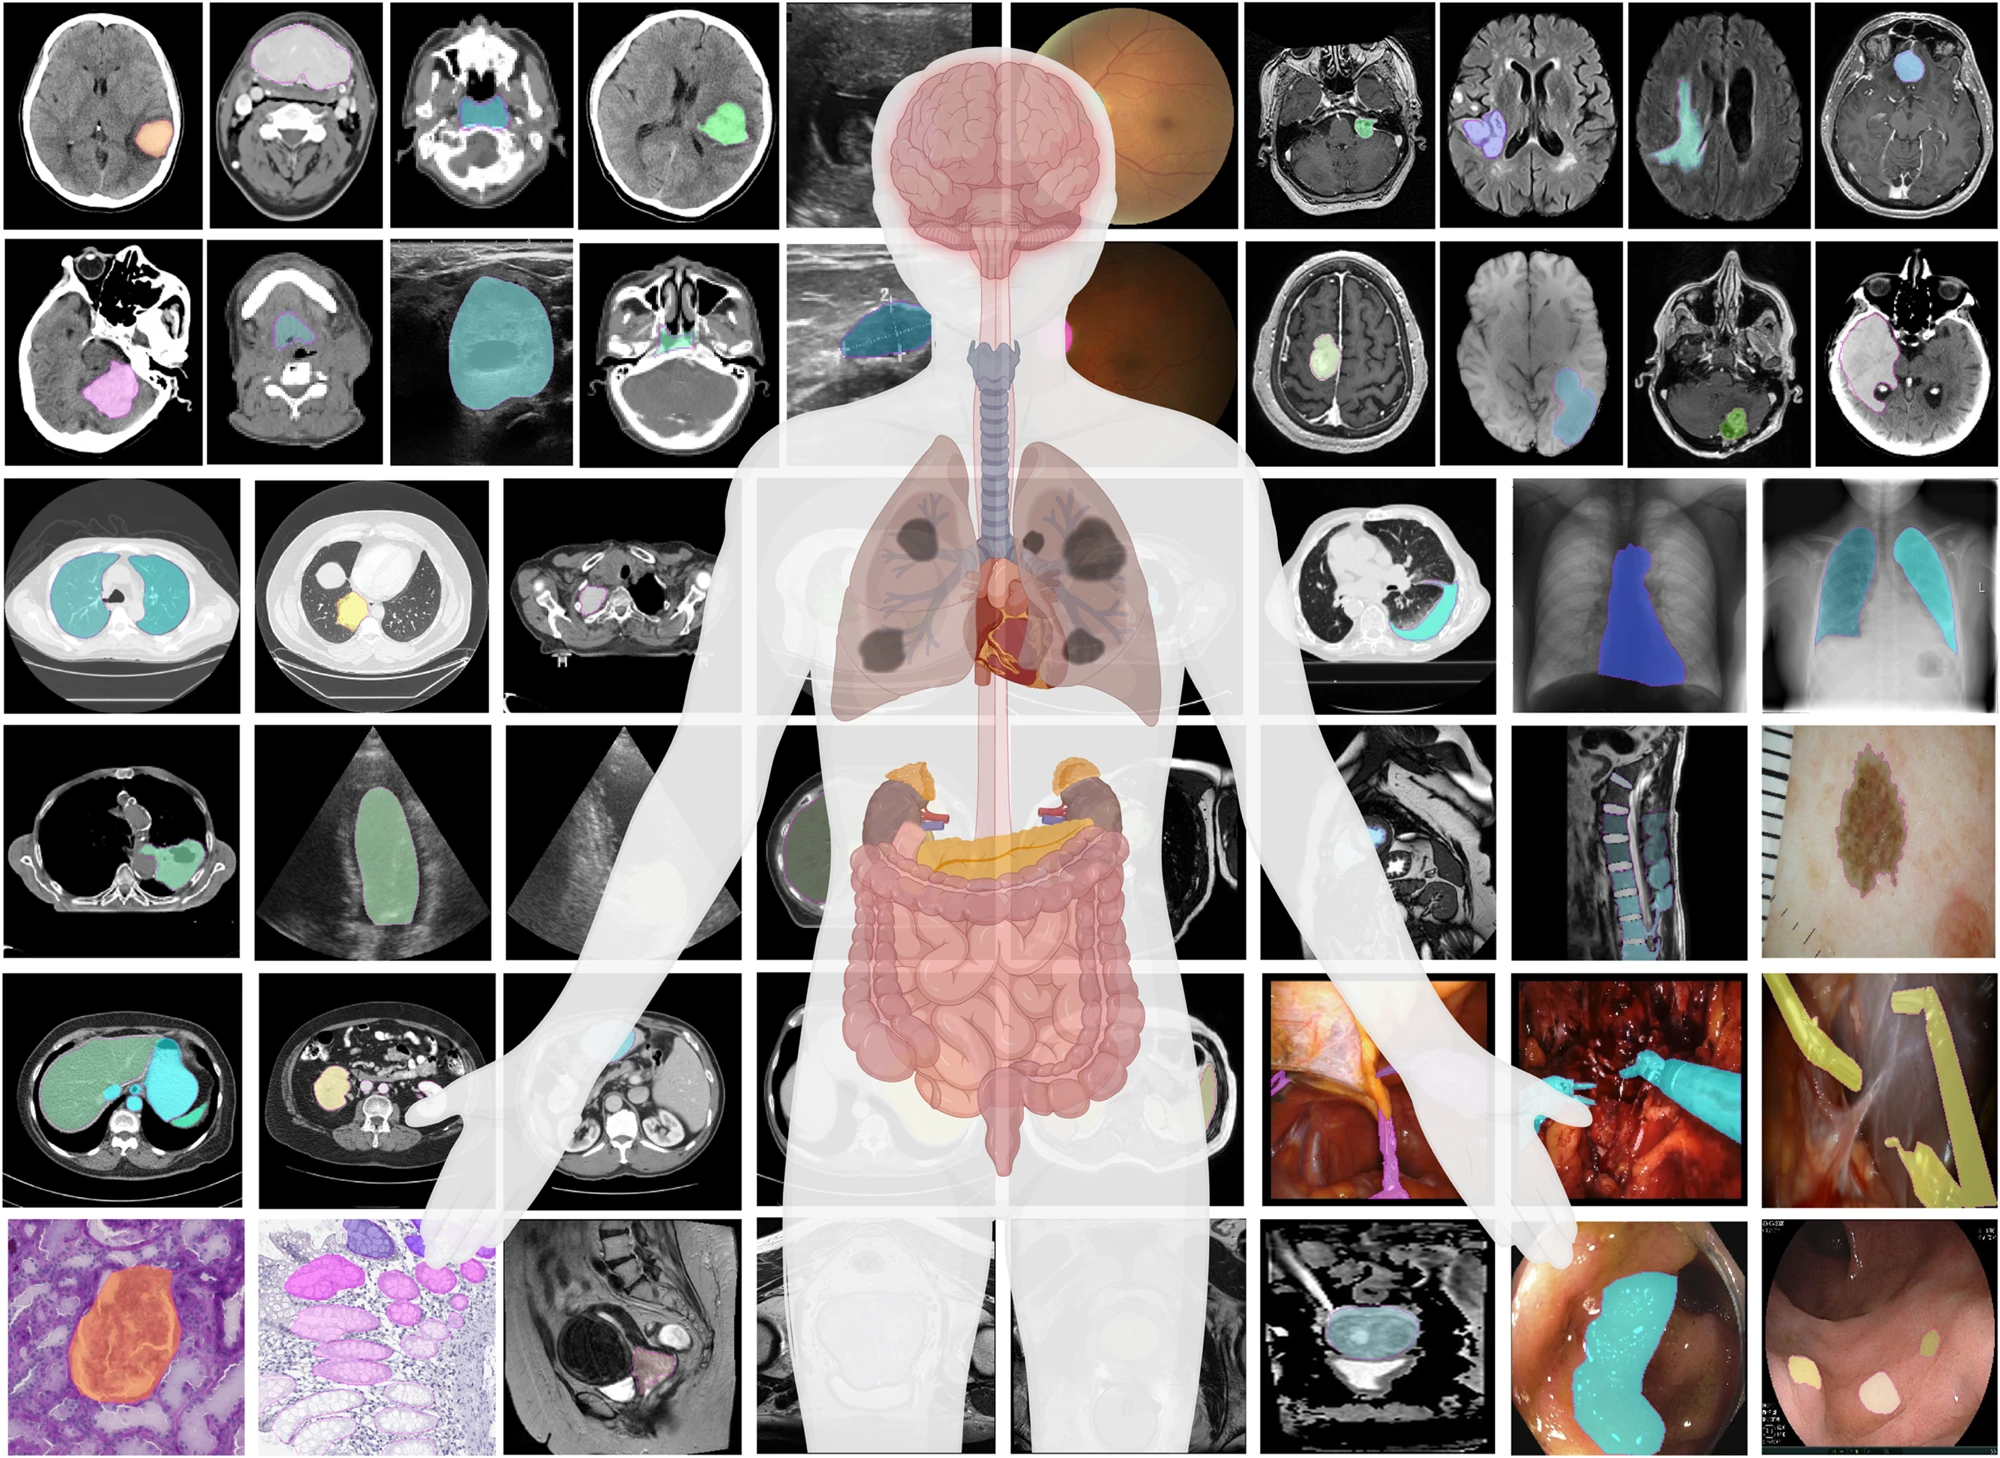
\includegraphics[width=\paperwidth, height=\paperheight]{images/segment_conv.png}%
        };
        % Semi-transparent orange banner at top
        \fill[orange1, opacity=0.82]
            (current page.north west) rectangle
            ([yshift=-1.2cm] current page.north east);
        % Title text
        \node[anchor=west, text=weiss, font=\large\bfseries, inner sep=0pt]
            at ([xshift=0.5cm, yshift=-0.6cm] current page.north west)
            {The Need for Segmentation};
        % Subtitle text
        \node[anchor=west, text=weiss, font=\small\mdseries, inner sep=0pt]
            at ([xshift=0.5cm, yshift=-1.0cm] current page.north west)
            {Why Automating Medical Image Analysis Matters};
        % Source attribution
        \node[anchor=south east, inner sep=4pt] at (current page.south east) {%
            {\tiny\textcolor{weiss}{Source: Mazurowski et al., \textit{Nature Communications} 15, 654 (2024). \url{https://doi.org/10.1038/s41467-024-44824-z}}}%
        };
    \end{tikzpicture}
\end{frame}

\subsection{Evolution of Deep Learning in Segmentation}
\begin{frame}
    \frametitle{Evolution of Deep Learning}
    \framesubtitle{From U-Net to Foundation Models}

    \centering
    \begin{tikzpicture}

        % horizontal backbone
        \draw[line width=2.5pt, orange1, -{Stealth[length=7pt]}] (-0.3,0) -- (11.8,0);

        % ---- U-Net ----
        \draw[fill=lila1, draw=lila1] (1.2,0) circle (6pt);
        \draw[lila1, line width=1pt] (1.2,0) -- (1.2,1.1);
        \node[draw=lila1, fill=lila1, rounded corners=4pt, minimum width=3.8cm,
              minimum height=1.1cm, align=center, font=\small, text=weiss, anchor=south]
              at (1.2,1.1) {\textbf{U-Net}\\[2pt]{\tiny Encoder-decoder + skip connections}};
        \node[draw=lila1, fill=lila1, rounded corners=2pt, minimum width=1cm,
              minimum height=0.42cm, font=\tiny\bfseries, text=weiss, anchor=north]
              at (1.2,-0.35) {2015};

        % ---- ViT / Swin ----
        \draw[fill=blau1, draw=blau1] (4.2,0) circle (6pt);
        \draw[blau1, line width=1pt] (4.2,0) -- (4.2,-1.1);
        \node[draw=blau1, fill=blau1, rounded corners=4pt, minimum width=3.8cm,
              minimum height=1.1cm, align=center, font=\small, text=weiss, anchor=north]
              at (4.2,-1.1) {\textbf{ViT / Swin}\\[2pt]{\tiny Global context, long-range deps.}};
        \node[draw=blau1, fill=blau1, rounded corners=2pt, minimum width=1cm,
              minimum height=0.42cm, font=\tiny\bfseries, text=weiss, anchor=south]
              at (4.2,0.35) {2020};

        % ---- Large-scale Pretraining ----
        \draw[fill=lila1, draw=lila1] (7.2,0) circle (6pt);
        \draw[lila1, line width=1pt] (7.2,0) -- (7.2,1.1);
        \node[draw=lila1, fill=lila1, rounded corners=4pt, minimum width=3.8cm,
              minimum height=1.1cm, align=center, font=\small, text=weiss, anchor=south]
              at (7.2,1.1) {\textbf{Pretraining}\\[2pt]{\tiny ImageNet, RadImageNet}};
        \node[draw=lila1, fill=lila1, rounded corners=2pt, minimum width=1cm,
              minimum height=0.42cm, font=\tiny\bfseries, text=weiss, anchor=north]
              at (7.2,-0.35) {2022};

        % ---- Foundation Models ----
        \draw[fill=blau1, draw=blau1] (10.2,0) circle (6pt);
        \draw[blau1, line width=1pt] (10.2,0) -- (10.2,-1.1);
        \node[draw=blau1, fill=blau1, rounded corners=4pt, minimum width=3.8cm,
              minimum height=1.1cm, align=center, font=\small, text=weiss, anchor=north]
              at (10.2,-1.1) {\textbf{Foundation Models}\\[2pt]{\tiny MedSAM, zero-shot inference}};
        \node[draw=blau1, fill=blau1, rounded corners=2pt, minimum width=1cm,
              minimum height=0.42cm, font=\tiny\bfseries, text=weiss, anchor=south]
              at (10.2,0.35) {2023};

    \end{tikzpicture}

    \vspace{0.6em}

    \begin{block}{}
        \centering
        Despite these advances the need for \textbf{manual annotation} remains a bottleneck.
    \end{block}

\end{frame}

\subsection{The Generalization Gap}

% figure macro — #1 = number of rows to show (1, 2, or 3)
\newcommand{\gengapfigure}[1]{%
\begin{tikzpicture}[
    train/.style={draw=orange1, fill=orange4, rounded corners=4pt,
                  minimum width=2.4cm, minimum height=0.8cm,
                  font=\small\bfseries, align=center, text=grau1},
    model/.style={draw=grau1, fill=grau4, rounded corners=4pt,
                  minimum width=1.9cm, minimum height=0.8cm,
                  font=\small\bfseries, align=center, text=grau1},
    fail/.style={draw=lila1, fill=lila1med, rounded corners=4pt,
                 minimum width=2.4cm, minimum height=0.8cm,
                 font=\small\bfseries, align=center, text=lila1},
    arr/.style={-{Stealth[length=5pt]}, grau2, line width=0.9pt},
    farr/.style={-{Stealth[length=5pt]}, lila1, line width=0.9pt, dashed},
    lbl/.style={font=\tiny, text=grau2, align=center}
]
    % Row 1 — always visible
    \node[train] (t1) {CT Scans\\{\tiny Hospital A}};
    \node[model, right=0.7cm of t1] (m1) {Trained\\Model};
    \node[fail, right=0.7cm of m1] (f1) {MRI Scans\\{\tiny Hospital B}};
    \draw[arr] (t1) -- (m1);
    \draw[farr] (m1) -- (f1);
    \node[text=lila1, font=\large\bfseries, right=0.15cm of f1] {$\times$};
    \node[lbl, above=0.12cm of t1] {Train};
    \node[lbl, above=0.12cm of f1] {Deploy};

    % Row 2 — visible from slide 2 onward
    \ifnum#1>1
        \node[train, below=0.8cm of t1] (t2) {Brain MRI\\{\tiny Tumour}};
        \node[model, right=0.7cm of t2] (m2) {Same\\Model};
        \node[fail, right=0.7cm of m2] (f2) {Cardiac MRI\\{\tiny New organ}};
        \draw[arr] (t2) -- (m2);
        \draw[farr] (m2) -- (f2);
        \node[text=lila1, font=\large\bfseries, right=0.15cm of f2] {$\times$};
    \fi

    % Row 3 — visible on slide 3 only
    \ifnum#1>2
        \node[train, below=0.8cm of t2] (t3) {Scanner A\\{\tiny 1.5T MRI}};
        \node[model, right=0.7cm of t3] (m3) {Same\\Model};
        \node[fail, right=0.7cm of m3] (f3) {Scanner B\\{\tiny 3T MRI}};
        \draw[arr] (t3) -- (m3);
        \draw[farr] (m3) -- (f3);
        \node[text=lila1, font=\large\bfseries, right=0.15cm of f3] {$\times$};
    \fi
\end{tikzpicture}%
}

\begin{frame}[t, label=gengap1]
    \frametitle{The Generalization Gap}
    \framesubtitle{Where the current model lacks}
    \begin{columns}[T]
        \column{0.43\textwidth}
            \vspace{0.6cm}
            \textcolor{orange1}{\textbf{Domain shift:}} Training data often fails when patient
            groups or imaging rules change.
        \column{0.54\textwidth}
            \centering
            \gengapfigure{1}
    \end{columns}
\end{frame}

\begin{frame}[t, label=gengap2]
    \frametitle{The Generalization Gap}
    \framesubtitle{Where the current model lacks}
    \begin{columns}[T]
        \column{0.43\textwidth}
            \vspace{0.6cm}
            \textcolor{orange1}{\textbf{Domain shift:}} Training data often fails when patient
            groups or imaging rules change.

            \vspace{0.6em}

            \textcolor{orange1}{\textbf{Modality shift:}} Models cannot switch between scan types
            like CT to MRI without being retrained.
        \column{0.54\textwidth}
            \centering
            \gengapfigure{2}
    \end{columns}
\end{frame}

\begin{frame}[t, label=gengap3]
    \frametitle{The Generalization Gap}
    \framesubtitle{Where the current model lacks}
    \begin{columns}[T]
        \column{0.43\textwidth}
            \vspace{0.6cm}
            \textcolor{orange1}{\textbf{Domain shift:}} Training data often fails when patient
            groups or imaging rules change.

            \vspace{0.6em}

            \textcolor{orange1}{\textbf{Modality shift:}} Models cannot switch between scan types
            like CT to MRI without being retrained.

            \vspace{0.6em}

            \textcolor{orange1}{\textbf{Site shift:}} Differences in hospital scanners and procedures
            lead to errors when using models at a new site.
        \column{0.54\textwidth}
            \centering
            \gengapfigure{3}
    \end{columns}

\end{frame}

\section{Related Works}
\begin{breakframe}
    Related Works
\end{breakframe}

\subsection{Medical Image Segmentation}
\begin{frame}[label=relworks1]
    \frametitle{Medical Image Segmentation}
    \framesubtitle{From Classical ML to Foundation Models}

    \begin{columns}[T]
        \column{0.48\textwidth}
            \vspace{0.3cm}
            \begin{itemize}\small
                \item Traditional ML lacked \textbf{\textcolor{orange1}{accuracy}} and \textbf{\textcolor{orange1}{scalability}}.

                \vspace{0.4em}
                \item \textbf{\textcolor{orange1}{Unsupervised}} methods partitioned images without prior labels.

                \vspace{0.4em}
                \item \textbf{\textcolor{orange1}{Supervised}} techniques relied on manually \textbf{\textcolor{orange1}{engineered features}}.
            \end{itemize}

        \column{0.48\textwidth}
            \vspace{0.3cm}
            \begin{itemize}\small
                \item \textbf{\textcolor{orange1}{Deep learning}} enabled automatic \textbf{\textcolor{orange1}{feature extraction}}.

                \vspace{0.4em}
                \item \textbf{\textcolor{orange1}{U-Net}} emerged as standard \textbf{\textcolor{orange1}{segmentation}} architecture.

                \vspace{0.4em}
                \item \textbf{\textcolor{orange1}{UniverSeg}} achieves high accuracy with minimal \textbf{\textcolor{orange1}{annotations}}.
            \end{itemize}

    \end{columns}

\end{frame}

\subsection{Semi-supervised Learning}
\begin{frame}[label=relworks2]
    \frametitle{Semi-supervised Learning}
    \framesubtitle{Leveraging Unlabeled Data to Bridge Annotation Gaps}

    \begin{columns}[T]
        \column{0.48\textwidth}
            \vspace{0.3cm}
            \begin{itemize}\small
                \item Uses \textbf{\textcolor{orange1}{unlabeled data}} for medical segmentation.

                \vspace{0.4em}
                \item Methods include \textbf{\textcolor{orange1}{self-training}} and \textbf{\textcolor{orange1}{co-training}}.

                \vspace{0.4em}
                \item \textbf{\textcolor{orange1}{4S}} extends masks to neighboring \textbf{\textcolor{orange1}{slices}}.
            \end{itemize}

        \column{0.48\textwidth}
            \vspace{0.3cm}
            \begin{itemize}\small
                \item 4S requires costly iterative model \textbf{\textcolor{orange1}{re-training}}.

                \vspace{0.4em}
                \item \textbf{\textcolor{orange1}{ICS}} uses efficient \textbf{\textcolor{orange1}{in-context learning}} instead.

                \vspace{0.4em}
                \item Avoids re-training reducing \textbf{\textcolor{orange1}{computational overhead}}.
            \end{itemize}

    \end{columns}

\end{frame}

\section{Method}
\begin{breakframe}
    Method
\end{breakframe}

\subsection{What is In-Context Learning}
\begin{frame}[label=method1]
    \frametitle{What is In-Context Learning?}

    \begin{columns}[T]
        \column{0.48\textwidth}
            \vspace{0.3cm}
            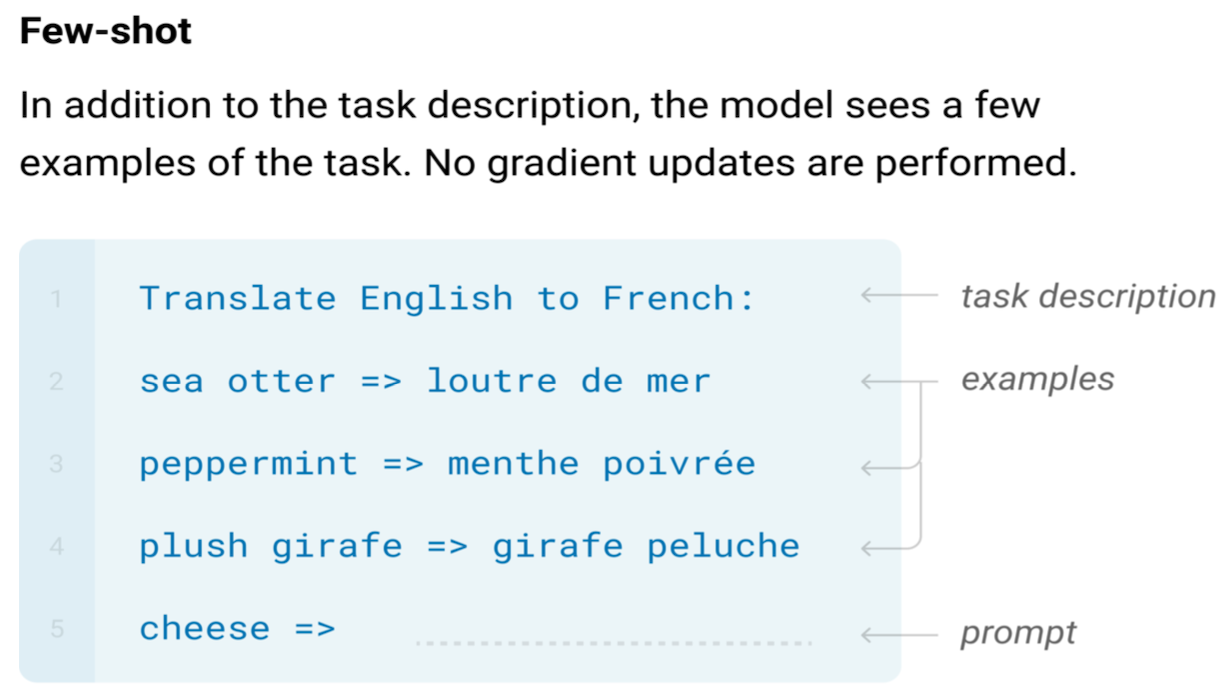
\includegraphics[width=\linewidth]{images/icl.png}

        \column{0.48\textwidth}
            \vspace{0.6cm}
            \begin{itemize}
                \item Provide examples directly in the prompt.

                \vspace{0.5em}
                \item No model weight updates required.

                \vspace{0.5em}
                \item Learns patterns directly at inference.
            \end{itemize}
    \end{columns}

\end{frame}

\subsection{Segmentation in Action}
\begin{frame}[label=method3a]
    \frametitle{The key difference with Universeg}
    \centering
    \includemedia[
        width=\textwidth,
        height=4.8cm,
        activate=pageopen,
        addresource=images/video.mp4,
        flashvars={
            source=images/video.mp4
            &autoPlay=true
            &loop=true
            &playCount=0
        }
    ]{}{VPlayer.swf}
    \vspace{0.3em}
    {\tiny\textcolor{grau2}{Source: \href{https://universeg.csail.mit.edu/assets/UVSWebstiteV5.mp4}{universeg.csail.mit.edu}}}
\end{frame}

\subsection{In-Context Learning Example}
\begin{frame}[label=method2]
    \frametitle{In-Context Learning for Segmentation}
    \framesubtitle{Pictorial Overview}

    \centering
    \begin{tikzpicture}[
        line/.style={line width=3.2pt, color=grau1},
        img/.style={inner sep=1.5pt, draw=grau3, line width=0.5pt},
        lbl/.style={font=\scriptsize\bfseries, text=grau1},
    ]

    \def\is{1.45cm}

    % ---- 2x2 support grid (vertical center = 0.85) ----
    \node[img] at (0.1,  1.7) {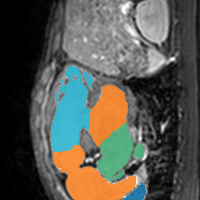
\includegraphics[width=\is,height=\is]{images/icl_ex1_ann.png}};
    \node[img] at (1.8,  1.7) {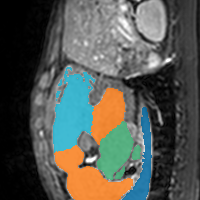
\includegraphics[width=\is,height=\is]{images/icl_ex2_ann.png}};
    \node[img] at (0.1,  0.0) {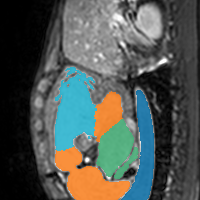
\includegraphics[width=\is,height=\is]{images/icl_ex3_ann.png}};
    \node[img] at (1.8,  0.0) {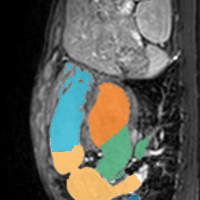
\includegraphics[width=\is,height=\is]{images/icl_ex4_ann.png}};
    \node[font=\small\bfseries, text=orange1, anchor=east] at (-0.7, 0.85) {ANNOTATED MASK};

    % ---- query image ----
    \node[img] at (0.95, -1.8) {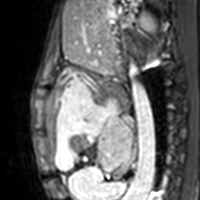
\includegraphics[width=\is,height=\is]{images/icl_query.png}};
    \node[font=\small\bfseries, text=grau1, anchor=east] at (-0.7, -1.8) {HEART SLICE};

    % ---- network (vertically centered at y=0.85) ----
    \node[inner sep=0pt] at (5.4, 0.85)
        {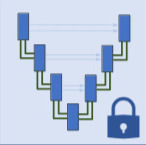
\includegraphics[width=2.9cm, height=2.9cm, keepaspectratio]{images/architect.jpg}};

    % ---- output box (same y=0.85) ----
    \node[draw=lila1, fill=schwarz, line width=1.5pt,
          minimum width=1.9cm, minimum height=1.9cm] at (9.0, 0.85) {};
    \node[font=\Large\bfseries, text=weiss] at (9.0, 0.85) {?};
    \node[font=\small\bfseries, text=lila1, anchor=north] at (9.0, -0.12) {PREDICTED MASK};

    % ---- horizontal: support set -> network ----
    \draw[line] (2.62, 0.85) -- (3.95, 0.85);

    % ---- L-shape: query -> network ----
    \draw[line] (1.75, -1.8) -- (5.52, -1.8);
    \draw[line] (5.46, -1.8) -- (5.46,  -0.57);

    % ---- horizontal: network -> output ----
    \draw[line] (6.85, 0.85) -- (8.05, 0.85);

    % ---- feedback loop: output -> annotated support set ----
    \draw[line] (9.0, 1.80) -- (9.0, 3.0);
    \draw[line] (9.054, 3.0)  -- (0.89, 3.0);
    \draw[line] (0.95, 3.0) -- (0.95, 2.48);

    \end{tikzpicture}

    \vspace{0.15em}
    {\tiny\textcolor{grau2}{Source: Manually created from HVSMR dataset}}

\end{frame}

\subsection{Univeral Segmentation Model (UniverSeg)}
\begin{frame}[label=method3]
    \frametitle{Univeral Segmentation Model (UniverSeg)}
    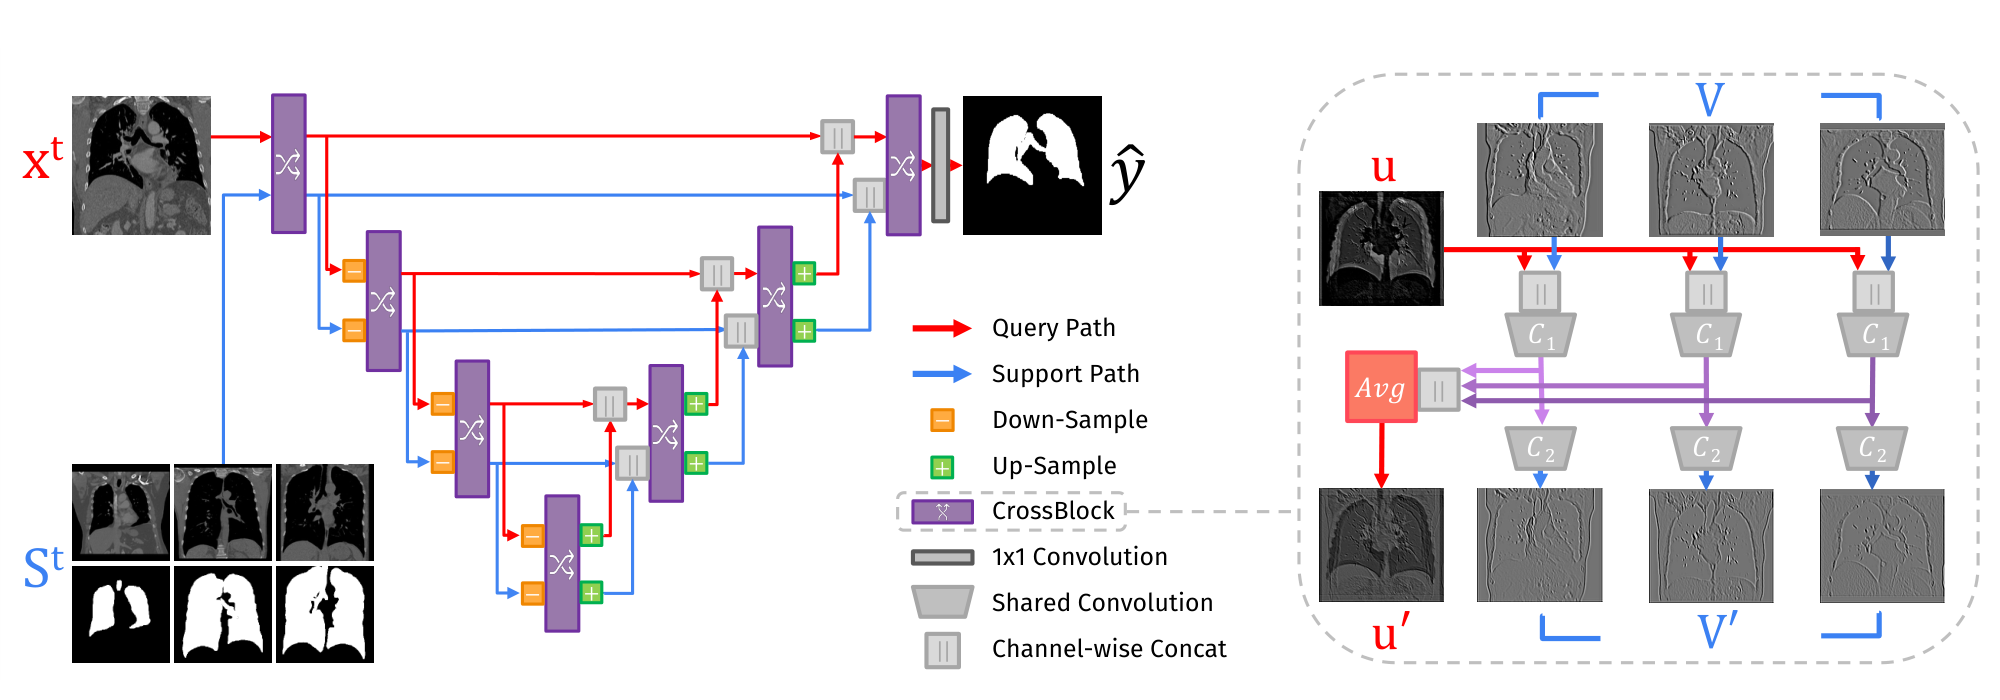
\includegraphics[width=1.0\linewidth, height=0.82\textheight, keepaspectratio]{images/Uniseg}

    {\tiny\textcolor{grau2}{Source: \href{https://universeg.csail.mit.edu/}{Butoi et al., UniverSeg: Universal Medical Image Segmentation, ICCV 2023}}}

\end{frame}

\subsection{ICS Architecture}
\begin{frame}[label=method4]
    \frametitle{ICS Architecture}

    \begin{tikzpicture}[remember picture, overlay]
        % Background image
        \node[anchor=center, yshift=-0.4cm] at (current page.center) {%
            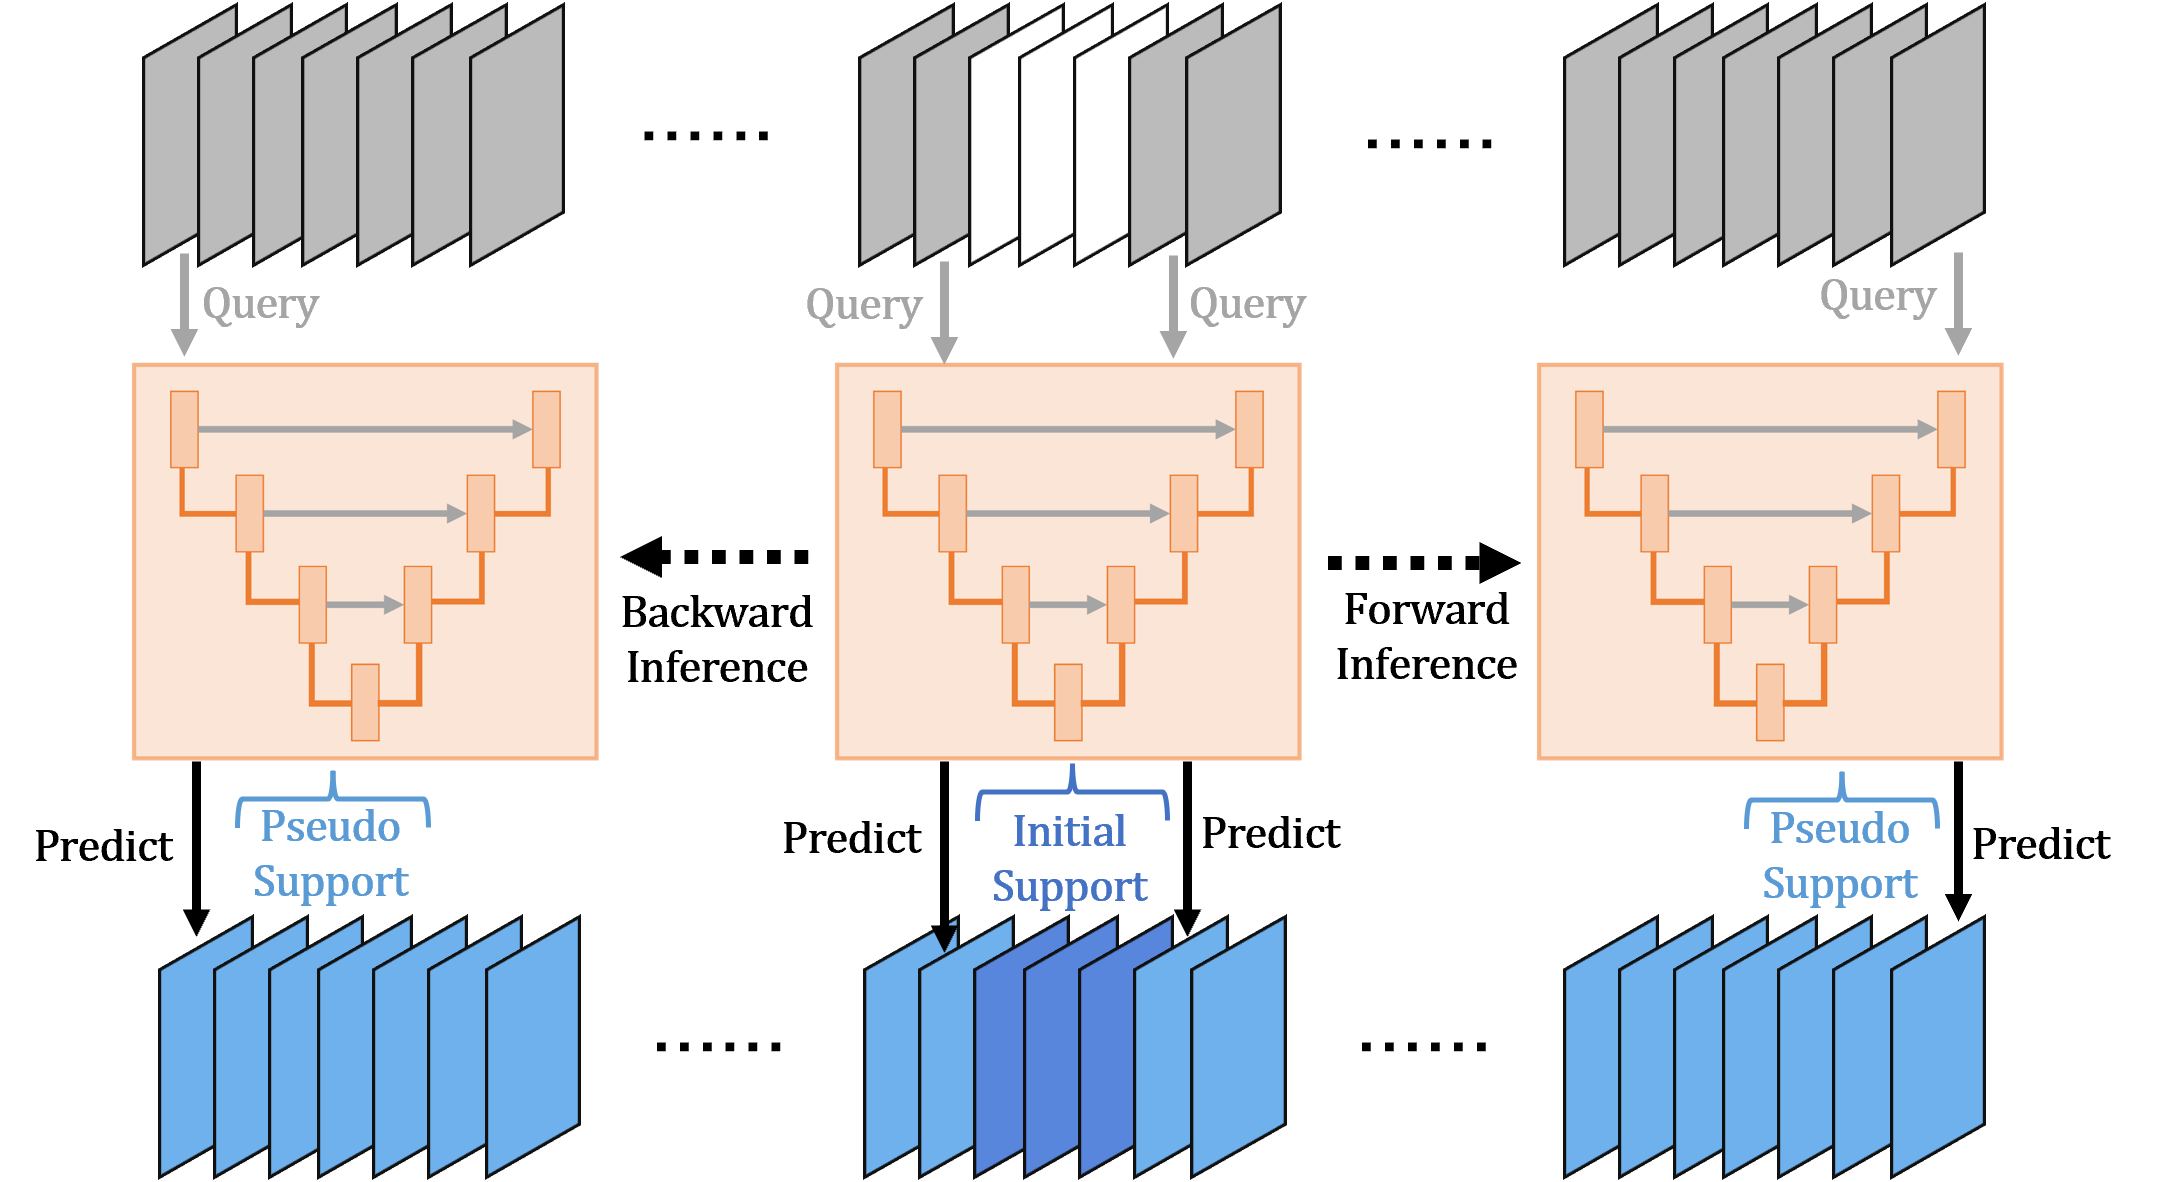
\includegraphics[width=0.80\textwidth]{fig2.png}%
        };
    \end{tikzpicture}

\end{frame}

\begin{frame}[label=method4b]
    \frametitle{ICS Architecture}
    \begin{tikzpicture}[remember picture, overlay]
        \node[anchor=center, yshift=-0.4cm] at (current page.center) {%
            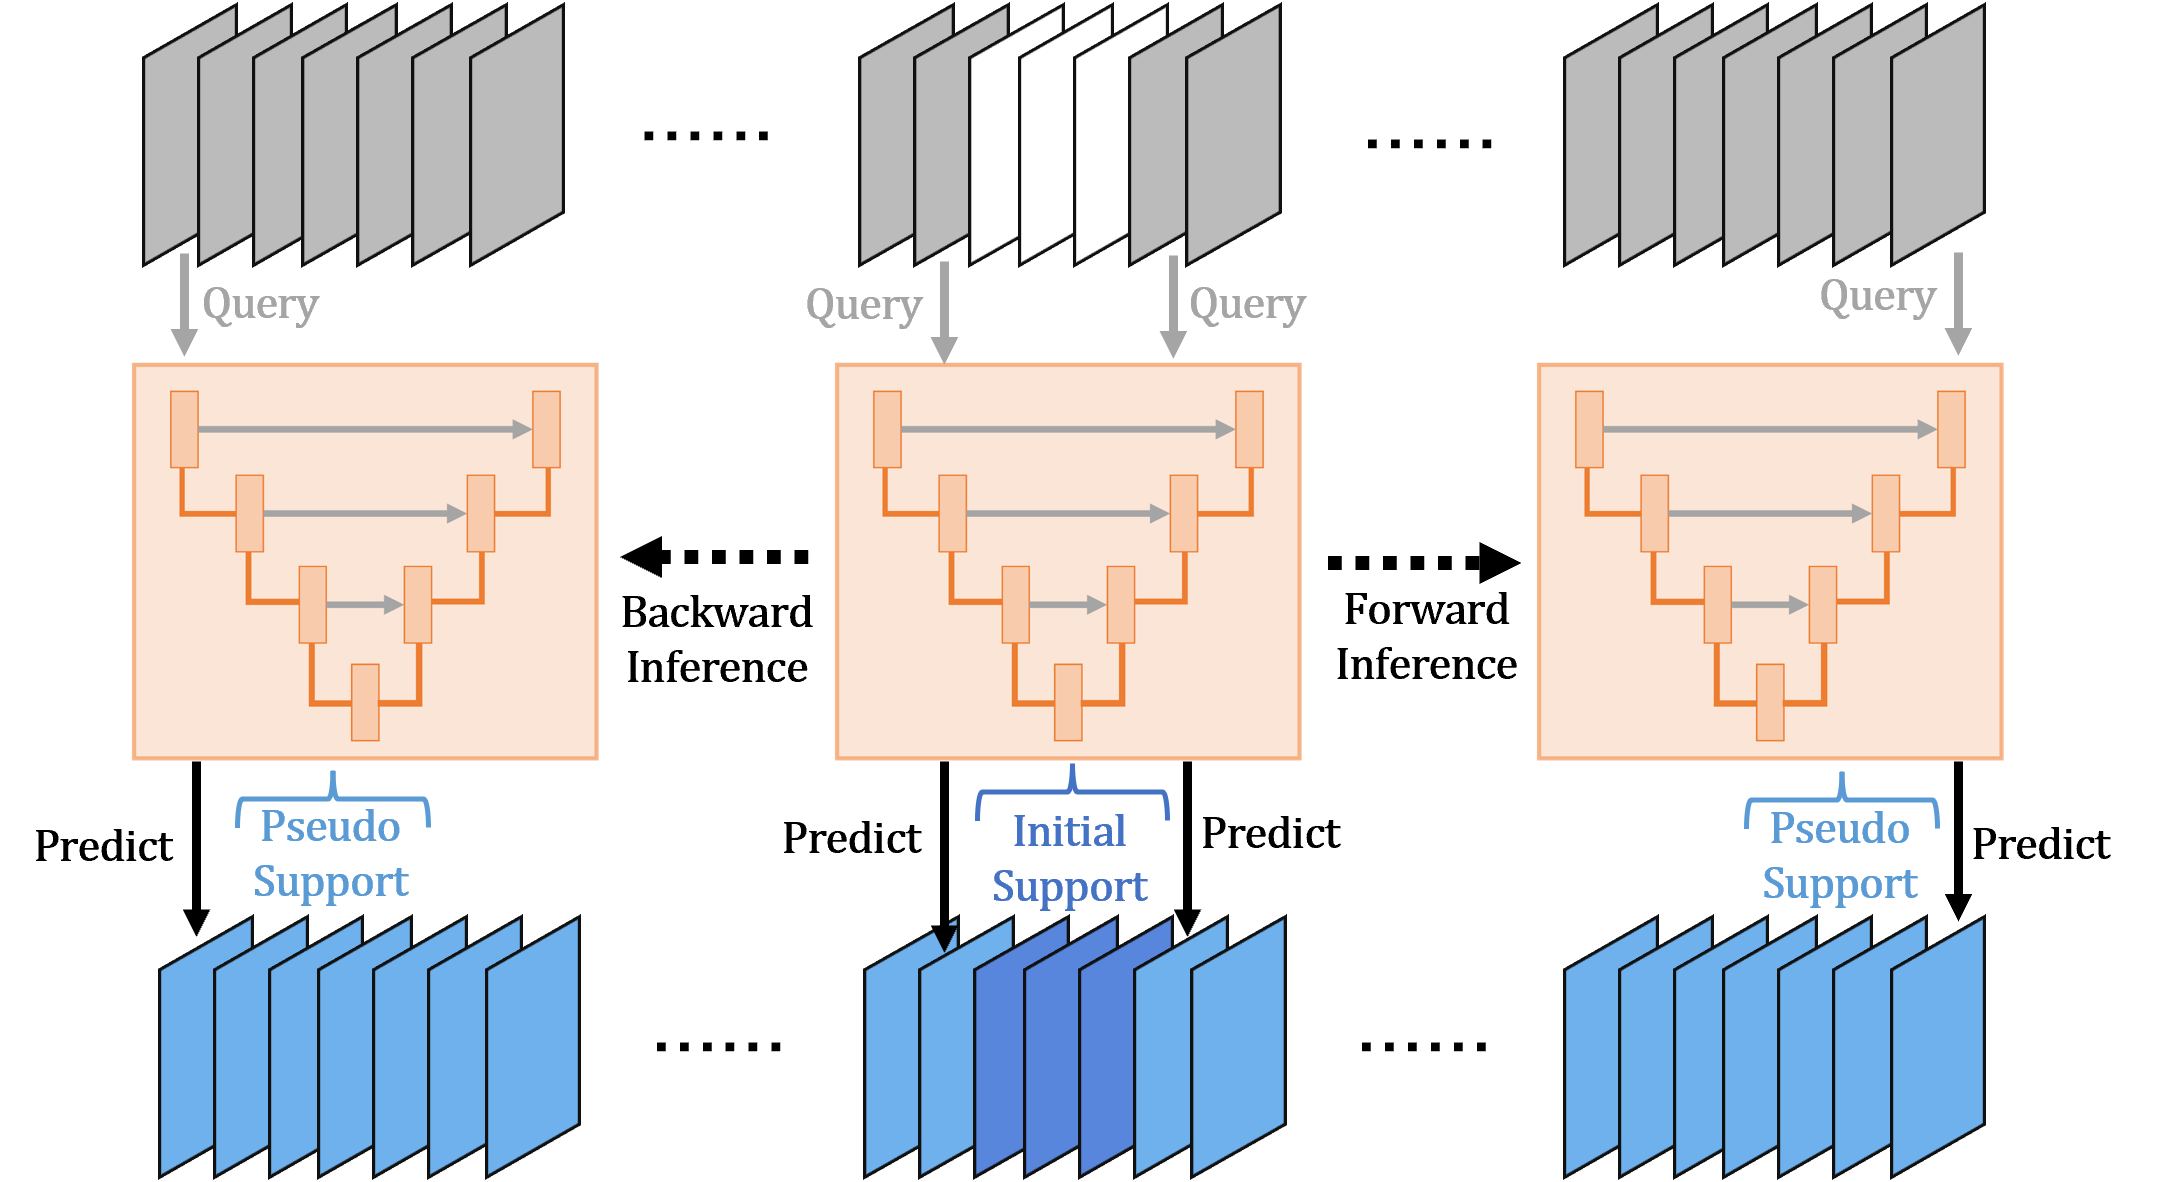
\includegraphics[width=0.80\textwidth]{fig2.png}%
        };
        % Box 1 — adjust xshift/yshift to move, change corner values to resize
        \draw[green!70!black, line width=2pt, rounded corners=3pt]
            ([xshift=1.4cm, yshift=3cm] current page.center)
            rectangle
            ([xshift=-1.5cm, yshift=-3.75cm] current page.center);
    \end{tikzpicture}

\end{frame}

\begin{frame}[label=method4c]
    \frametitle{ICS Architecture}
    \begin{tikzpicture}[remember picture, overlay]
        \node[anchor=center, yshift=-0.4cm] at (current page.center) {%
            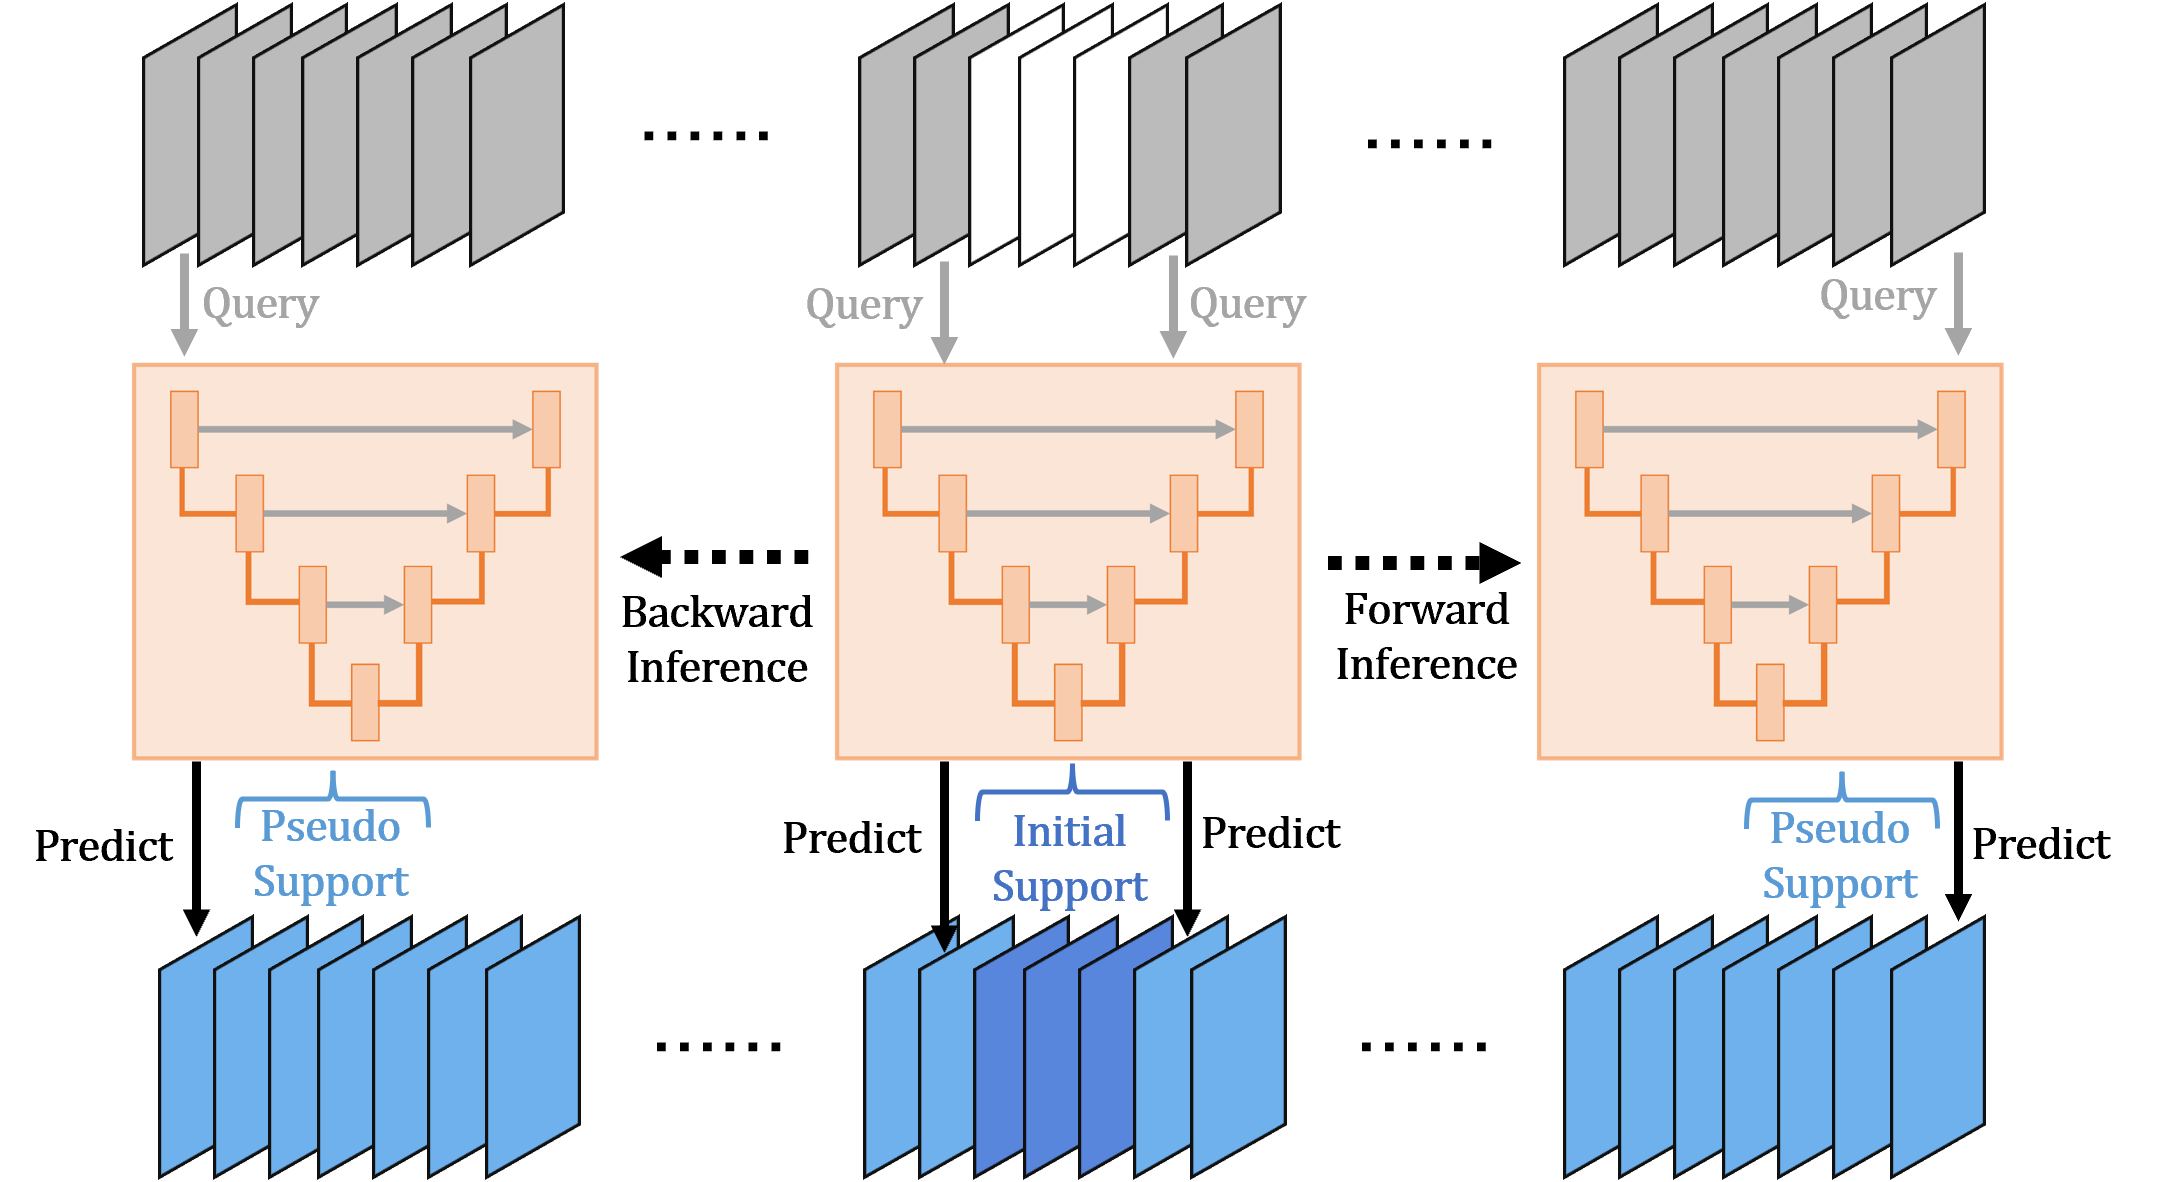
\includegraphics[width=0.80\textwidth]{fig2.png}%
        };
        % Box 2 — right side
        \draw[green!70!black, line width=2pt, rounded corners=3pt]
            ([xshift=2.4cm, yshift=3cm] current page.center)
            rectangle
            ([xshift=5.7cm, yshift=-3.75cm] current page.center);
    \end{tikzpicture}

\end{frame}

\begin{frame}[label=method4d]
    \frametitle{ICS Architecture}
    \begin{tikzpicture}[remember picture, overlay]
        \node[anchor=center, yshift=-0.4cm] at (current page.center) {%
            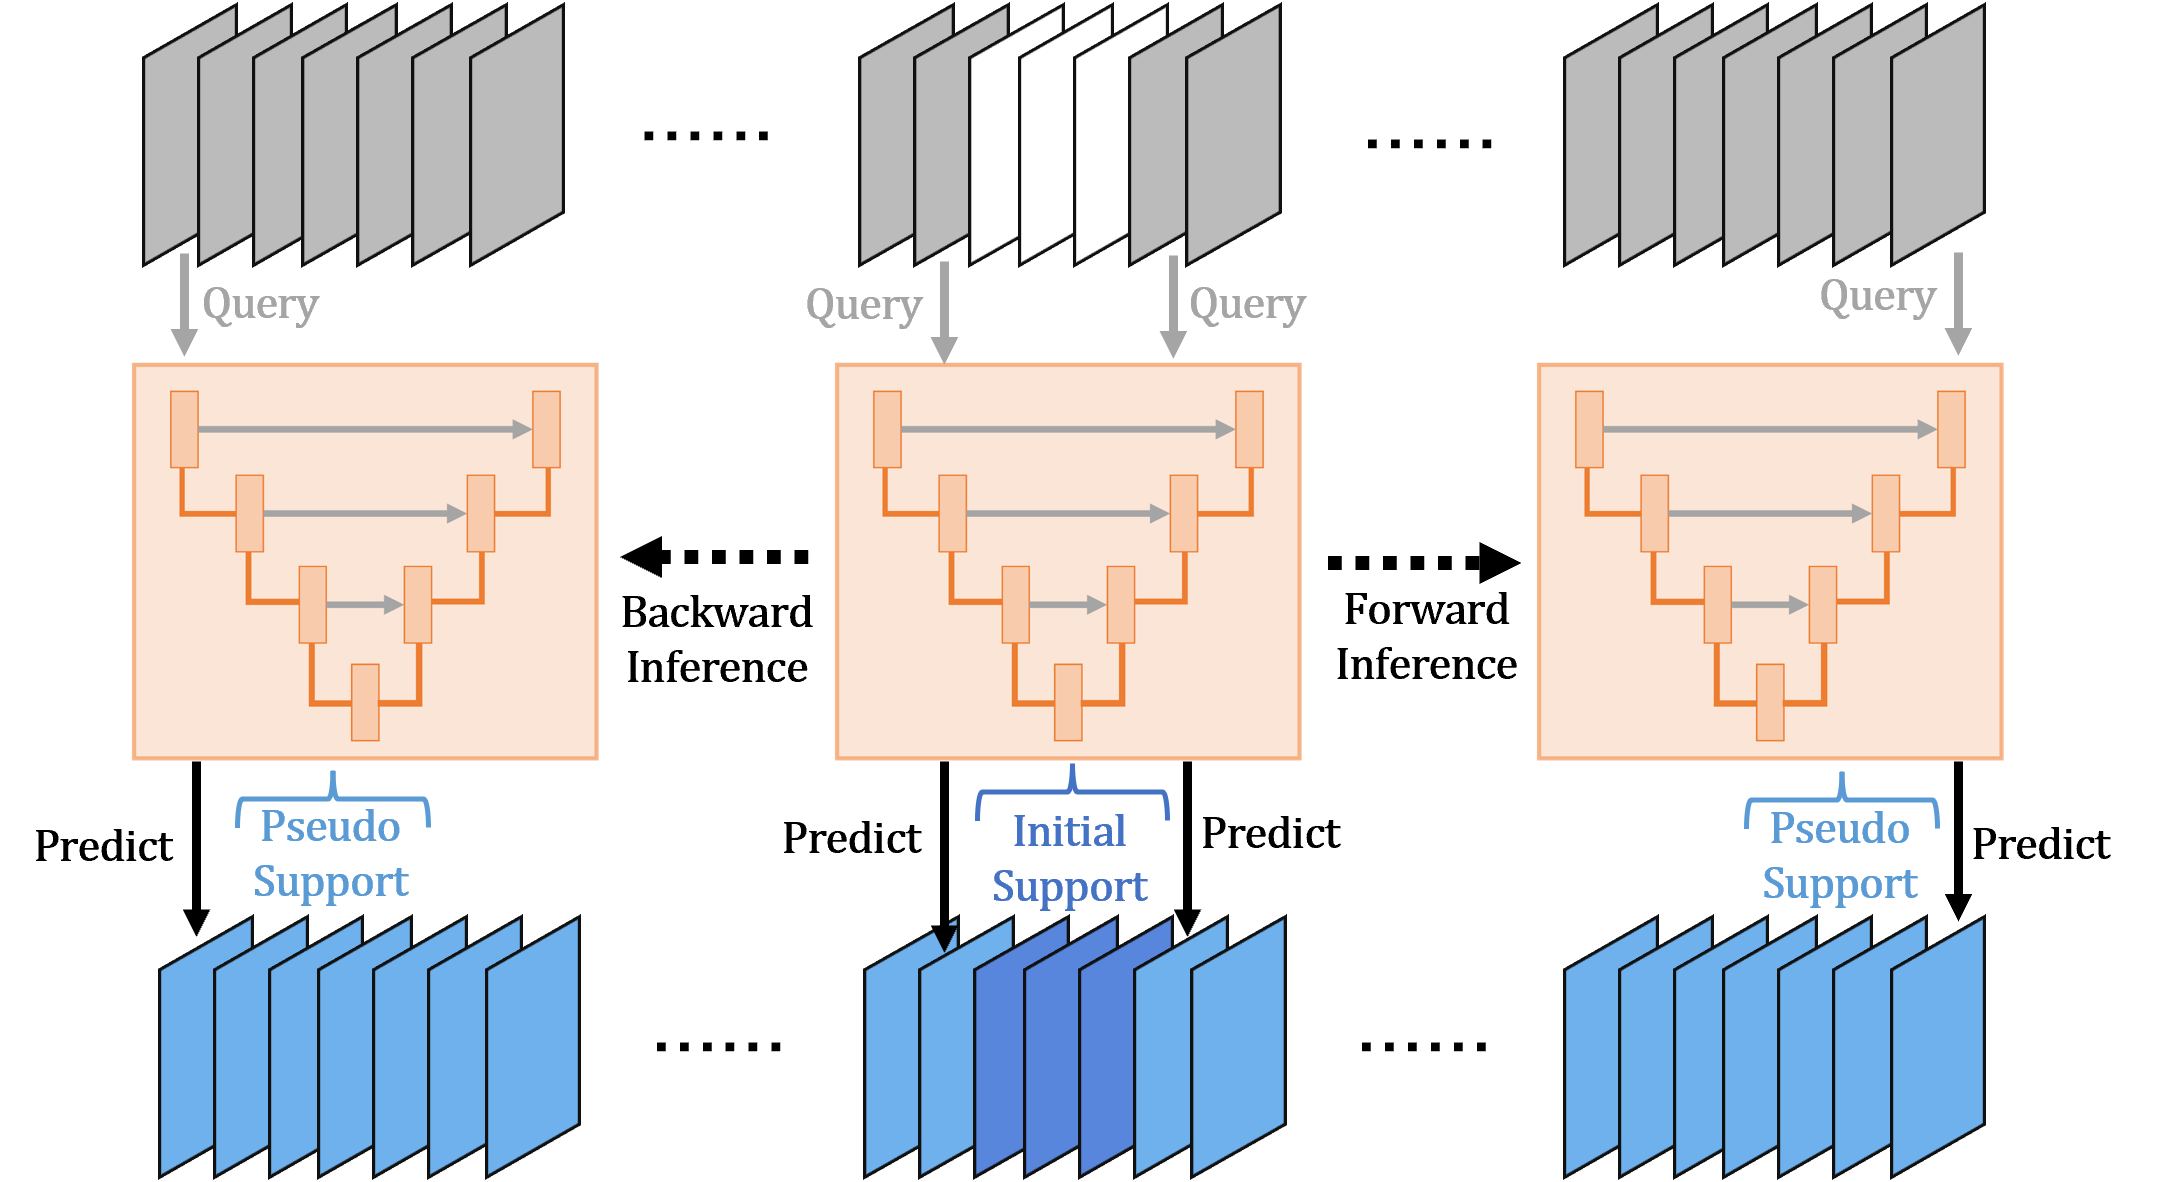
\includegraphics[width=0.80\textwidth]{fig2.png}%
        };
        % Box 3 — left most
        \draw[green!70!black, line width=2pt, rounded corners=3pt]
            ([xshift=-5.9cm, yshift=3cm] current page.center)
            rectangle
            ([xshift=-2.6cm, yshift=-3.75cm] current page.center);
    \end{tikzpicture}

\end{frame}

\subsection{Problem Formulation}
\begin{frame}[t, label=method5]
    \frametitle{Problem Formulation}
    \framesubtitle{Implementation of ICS }
    \vspace{-0.1cm}
    We consider a volumetric dataset where each $\text{slice}_k$
    ($1 \le k \le n$) is a 2D cross-sectional image from CT or MRI:
    \[
        V = \{\text{slice}_1,\, \text{slice}_2,\, \ldots,\, \text{slice}_n\}
    \]

    Only $m$ slices have ground-truth labels forming the
    \textcolor{orange1}{\textbf{support set}} $S$:
    \vspace{-0.1cm}   
    \[
        S = \bigl\{(\text{slice}_{\ell_1}, \text{label}_{\ell_1}),\;
                   (\text{slice}_{\ell_2}, \text{label}_{\ell_2}),\;
                   \ldots,\;
                   (\text{slice}_{\ell_m}, \text{label}_{\ell_m})\bigr\}
    \]
    \vspace{-0.1cm}
    where $\ell_1, \ell_2, \ldots, \ell_m$ are the labeled slice indices satisfying
    $1 \le \ell_1 < \ell_2 < \cdots < \ell_m \le n$.

\end{frame}

\begin{frame}[t, label=method5b]
    \frametitle{Problem Formulation}
    \framesubtitle{Implementation of ICS }
    \vspace{-0.1cm}
    We consider a volumetric dataset where each $\text{slice}_k$
    ($1 \le k \le n$) is a 2D cross-sectional image from CT or MRI:
    \[
        V = \{\text{slice}_1,\, \text{slice}_2,\, \ldots,\, \text{slice}_n\}
    \]

    Only $m$ slices have ground-truth labels forming the
    \textcolor{orange1}{\textbf{support set}} $S$:
    \vspace{-0.1cm}  

    \[
        S = \bigl\{(\text{slice}_{\ell_1}, \text{label}_{\ell_1}),\;
                   (\text{slice}_{\ell_2}, \text{label}_{\ell_2}),\;
                   \ldots,\;
                   (\text{slice}_{\ell_m}, \text{label}_{\ell_m})\bigr\}
    \]
    \vspace{-0.1cm}
    where $\ell_1, \ell_2, \ldots, \ell_m$ are the labeled slice indices satisfying
    $1 \le \ell_1 < \ell_2 < \cdots < \ell_m \le n$.

    \vspace{0.3em}

    \textbf{Objective:} generate masks for all remaining $(n - m)$ unlabeled slices
    $k \in \{1,\ldots,n\} \setminus \{\ell_1,\ldots,\ell_m\}$:
    \[
        \hat{M}_k = f\!\left(\text{slice}_k,\; S\right)
    \]

    Here $f$ is the pretrained \textcolor{orange1}{\textbf{UniverSeg}} model.\textsuperscript{[1,7]}
    $\hat{M}_k$ has the same dimensions as $\text{slice}_k$ and assigns each pixel
    to its most likely anatomical class or background.

    \vspace{0.3em}
    {\tiny\textcolor{grau2}{Sources: \href{https://arxiv.org/abs/2412.13299}{Takaya \& Yamamoto, 2025} \quad \href{https://universeg.csail.mit.edu/}{Butoi et al., 2023}}}

\end{frame}

\subsection{Forward and Backward Inference}
\begin{frame}[label=method6]
    \frametitle{Forward \& Backward Inference}
    \framesubtitle{How ICS Propagates Through the Volume}

    \begin{tikzpicture}[remember picture, overlay]
        \node[anchor=center, yshift=-0.4cm] at (current page.center) {%
            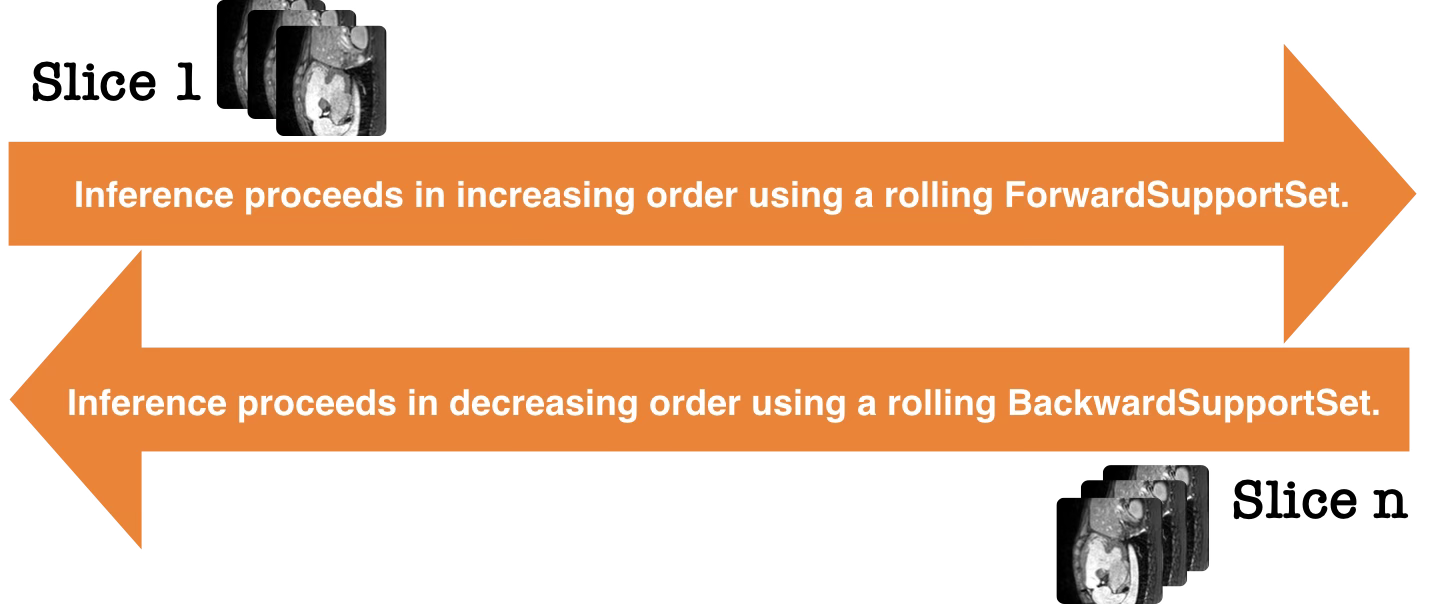
\includegraphics[width=0.96\paperwidth, height=0.82\paperheight, keepaspectratio]{images/inference.png}%
        };
    \end{tikzpicture}

\end{frame}

\section{Dataset \& Experiments}
\begin{breakframe}
    Experiments
\end{breakframe}

\subsection{Dataset}
\begin{frame}[label=current]
    \frametitle{The HVSMR Dataset}
    \framesubtitle{How our heart looks visually }

    \begin{columns}[c]
        \column{0.52\textwidth}
            \vspace{0.2cm}
            \begin{columns}[c]
                \column{0.33\textwidth}
                    \centering
                    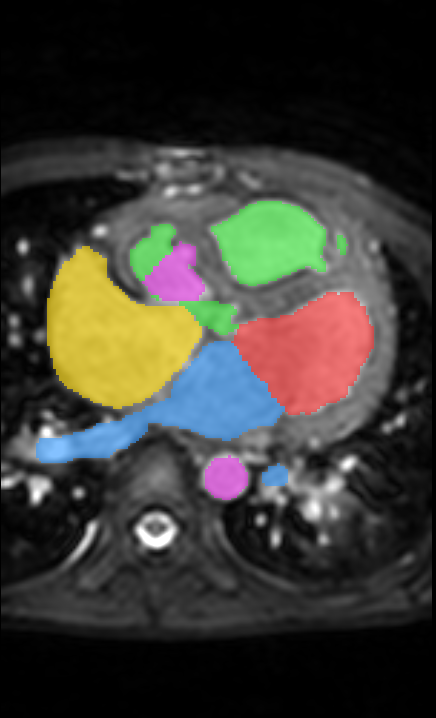
\includegraphics[width=\linewidth]{images/axial.png}
                \column{0.33\textwidth}
                    \centering
                    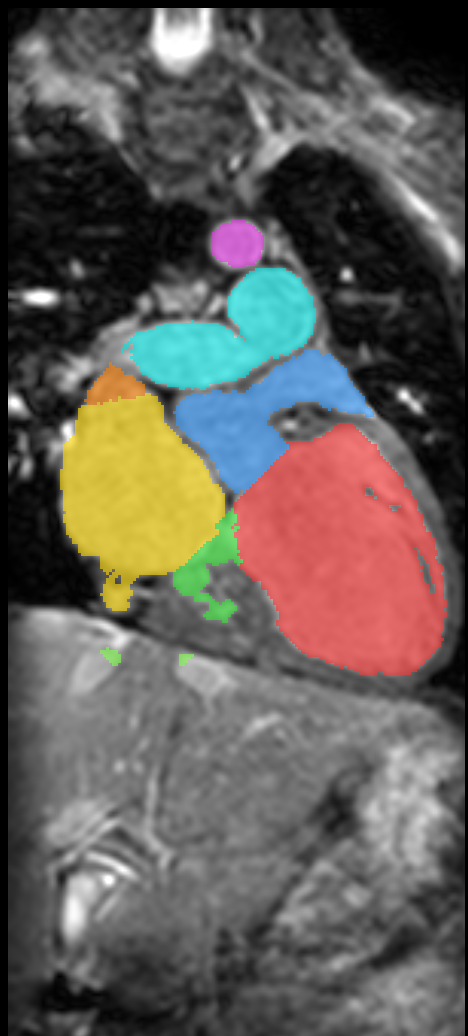
\includegraphics[width=\linewidth]{images/coronal.png}
                \column{0.33\textwidth}
                    \centering
                    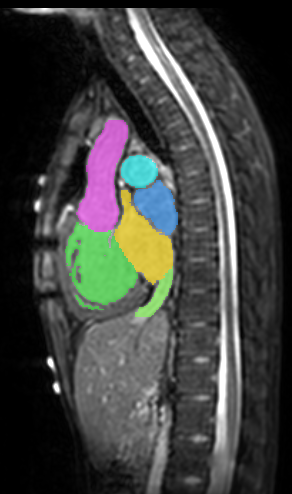
\includegraphics[width=\linewidth]{images/sagittal.png}
            \end{columns}

        \column{0.44\textwidth}
            \centering
            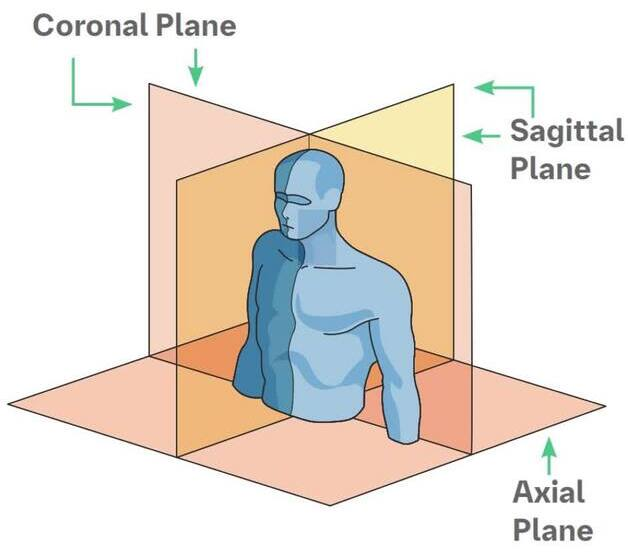
\includegraphics[width=\linewidth, height=0.78\textheight, keepaspectratio]{images/view.jpg}

    \end{columns}

\end{frame}

\subsection{8 Cardiac Regions}
\begin{frame}
    \frametitle{8 Cardiac Regions}
    \framesubtitle{3D Visualization of Heart regions}

    \makebox[\textwidth][l]{\hspace*{-0.5cm}%
    \begin{columns}[c]

        % LEFT COLUMN — Pair 1 and Pair 3
        \column{0.5\textwidth}

            % Pair 1
            \begin{columns}[c]
                \column{0.65\textwidth}
                    \animategraphics[loop, autoplay, width=\linewidth]{15}{SlicerCapture/pair1/image_}{00000}{00119}
                \column{0.35\textwidth}
                    {\small\textcolor{red}{\rule{0.7em}{0.7em}}~Left Ventricle}\\[0.4em]
                    {\small\textcolor{orange1}{\rule{0.7em}{0.7em}}~Aorta}
            \end{columns}

            \vspace{0.4em}

            % Pair 3
            \begin{columns}[c]
                \column{0.65\textwidth}
                    \animategraphics[loop, autoplay, width=\linewidth]{15}{SlicerCapture/pair3/image_}{00000}{00119}
                \column{0.35\textwidth}
                    {\small\textcolor[rgb]{0.95,0.45,0.65}{\rule{0.7em}{0.7em}}~Left Atrium}\\[0.4em]
                    {\small\textcolor{cyan1}{\rule{0.7em}{0.7em}}~Right Atrium}
            \end{columns}

        % RIGHT COLUMN — Pair 2 and Pair 4
        \column{0.5\textwidth}

            % Pair 2
            \begin{columns}[c]
                \column{0.65\textwidth}
                    \animategraphics[loop, autoplay, width=\linewidth]{15}{SlicerCapture/pair2/image_}{00000}{00119}
                \column{0.35\textwidth}
                    {\small\textcolor{blau1}{\rule{0.7em}{0.7em}}~Right Ventricle}\\[0.4em]
                    {\small\textcolor{gruen1}{\rule{0.7em}{0.7em}}~Pulmonary Artery}
            \end{columns}

            \vspace{0.4em}

            % Pair 4
            \begin{columns}[c]
                \column{0.65\textwidth}
                    \animategraphics[loop, autoplay, width=\linewidth]{15}{SlicerCapture/pair4/image_}{00000}{00119}
                \column{0.35\textwidth}
                    {\small\textcolor{lila1}{\rule{0.7em}{0.7em}}~Superior Vena Cava}\\[0.4em]
                    {\small\textcolor[rgb]{0.9,0.8,0.05}{\rule{0.7em}{0.7em}}~Inferior Vena Cava}
            \end{columns}

    \end{columns}}

\end{frame}

\subsection{Experimental Settings}
\begin{frame}[label=expsettings]
    \frametitle{Experimental Settings}
    \framesubtitle{Three Evaluation Protocols}

    \begin{columns}[T]

        \column{0.30\textwidth}
            \begin{block}{Quantitative \& Qualitative}
                Compares ICS against baseline UniverSeg using identical support
                slices and augmentation settings to assess accuracy and boundary quality.
            \end{block}

        \column{0.02\textwidth}

        \column{0.30\textwidth}
            \begin{block}{Support Slice Count}
                Evaluates how varying initial support slices ($m = 1$ to $5$)
                affects performance and identifies diminishing returns.
            \end{block}

        \column{0.02\textwidth}

        \column{0.30\textwidth}
            \begin{block}{Initial Slice Position}
                Investigates how spatial positioning of labeled slices influences
                segmentation using Patient\_32 as representative case.
            \end{block}

    \end{columns}

\end{frame}

\subsection{Dice Similarity Coefficient}
\begin{frame}[label=dscslide2]
    \frametitle{Dice Similarity Coefficient}
    \framesubtitle{Primary Evaluation Metric}

    \begin{columns}[c]
        \column{0.55\textwidth}
            \centering
            \begin{tikzpicture}[scale=1.05]
                % background
                \fill[grau3!40] (-3.2,-2.2) rectangle (3.6,2.5);

                % left circle — Segmentation (#E53935)
                \fill[vennred, opacity=0.88] (-0.7,0) circle (1.8cm);
                % right circle — Ground Truth (#43A047)
                \fill[venngreen, opacity=0.88] (0.7,0) circle (1.8cm);
                % overlap — True Positive (#1E88E5)
                \begin{scope}
                    \clip (-0.7,0) circle (1.8cm);
                    \fill[vennblue, opacity=0.95] (0.7,0) circle (1.8cm);
                \end{scope}

                % TN label outside both circles
                \node[font=\large\bfseries, text=grau1] at (-2.6, 2) {TN};

                % FP label
                \node[font=\large\bfseries, text=weiss] at (-1.7, 0) {FP};

                % TP label
                \node[font=\large\bfseries, text=weiss] at (0.0, 0) {TP};

                % FN label
                \node[font=\large\bfseries, text=weiss] at (1.6, 0) {FN};

            \end{tikzpicture}

        \column{0.41\textwidth}
            \vspace{0.5cm}
            \[\displaystyle
                \text{DSC} = \frac{2 \cdot \text{TP}}{2 \cdot \text{TP} + \text{FP} + \text{FN}}
            \]

            \vspace{0.6em}
            \textcolor{vennred}{\rule{0.8em}{0.8em}}~Predicted Mask\\[6pt]
            \textcolor{venngreen}{\rule{0.8em}{0.8em}}~Ground Truth

            \vspace{0.6em}
            \begin{exampleblock}{}
                \centering DSC = 1 \quad perfect overlap\\[4pt]
                DSC = 0 \quad no overlap
            \end{exampleblock}

    \end{columns}

\end{frame}

\section{Results}
\begin{breakframe}
    Results
\end{breakframe}

\subsection{Quantitative Results}
\begin{frame}[t, label=quantresults]
    \frametitle{Quantitative Results}
    \framesubtitle{Dice Similarity Coefficient Table}

    % Adjust this negative value to move the block further up or down
    \vspace*{-0.15cm}

    \begin{columns}[c]

        \column{0.05\textwidth}

        \column{0.40\textwidth}
            
            \centering
            {\scriptsize
            \setlength{\arrayrulewidth}{0.8pt}
            \begin{tabular}{>{\bfseries}l ccc cc}
                \toprule
                \multicolumn{1}{l}{Region} & \multicolumn{2}{c}{Baseline} & \multicolumn{2}{c}{ICS} & p-value \\
                \cmidrule(lr){2-3}\cmidrule(lr){4-5}
                & Mean & Std & Mean & Std & \\
                \midrule
                \textcolor{red}{\rule{0.5em}{0.5em}}~LV
                    & 0.5489 & 0.0893 & \textcolor{orange1}{0.5475} & 0.0770 & 0.8903 \\[2pt]
                \textcolor{blau1}{\rule{0.5em}{0.5em}}~RV
                    & 0.4663 & 0.1047 & \textcolor{orange1}{0.4741} & 0.0933 & 0.3820 \\[2pt]
                \textcolor[rgb]{0.95,0.45,0.65}{\rule{0.5em}{0.5em}}~LA
                    & 0.3879 & 0.1210 & \textbf{0.4272} & 0.0925 & 0.0007 \\[2pt]
                \textcolor{cyan1}{\rule{0.5em}{0.5em}}~RA
                    & 0.5500 & 0.1191 & \textbf{0.5734} & 0.0791 & 0.0214 \\[2pt]
                \textcolor{orange1}{\rule{0.5em}{0.5em}}~AO
                    & 0.4945 & 0.1269 & \textbf{0.5210} & 0.0679 & 0.0206 \\[2pt]
                \textcolor{gruen1}{\rule{0.5em}{0.5em}}~PA
                    & 0.3807 & 0.1336 & \textbf{0.4745} & 0.0974 & $<$0.0001 \\[2pt]
                \textcolor{lila1}{\rule{0.5em}{0.5em}}~SVC
                    & 0.4079 & 0.1805 & \textbf{0.4938} & 0.1226 & $<$0.0001 \\[2pt]
                \textcolor[rgb]{0.9,0.8,0.05}{\rule{0.5em}{0.5em}}~IVC
                    & 0.4607 & 0.1258 & \textcolor{orange1}{0.4629} & 0.0871 & 0.8561 \\
                \bottomrule
            \end{tabular}
            }

        \column{0.55\textwidth}
            \begin{center}
            \hspace*{1.7cm}
            \animategraphics[loop, autoplay, width=0.75\linewidth]{15}{SlicerCapture/cropped/image_}{00000}{00119}
            \end{center}

    \end{columns}

\end{frame}

\subsection{Qualitative Results}
\begin{frame}
    \frametitle{Qualitative Results}
    \framesubtitle{Segmentated LV and PA Regions respectivley }

    \begin{columns}[c]
        \column{0.45\textwidth}
            \centering
            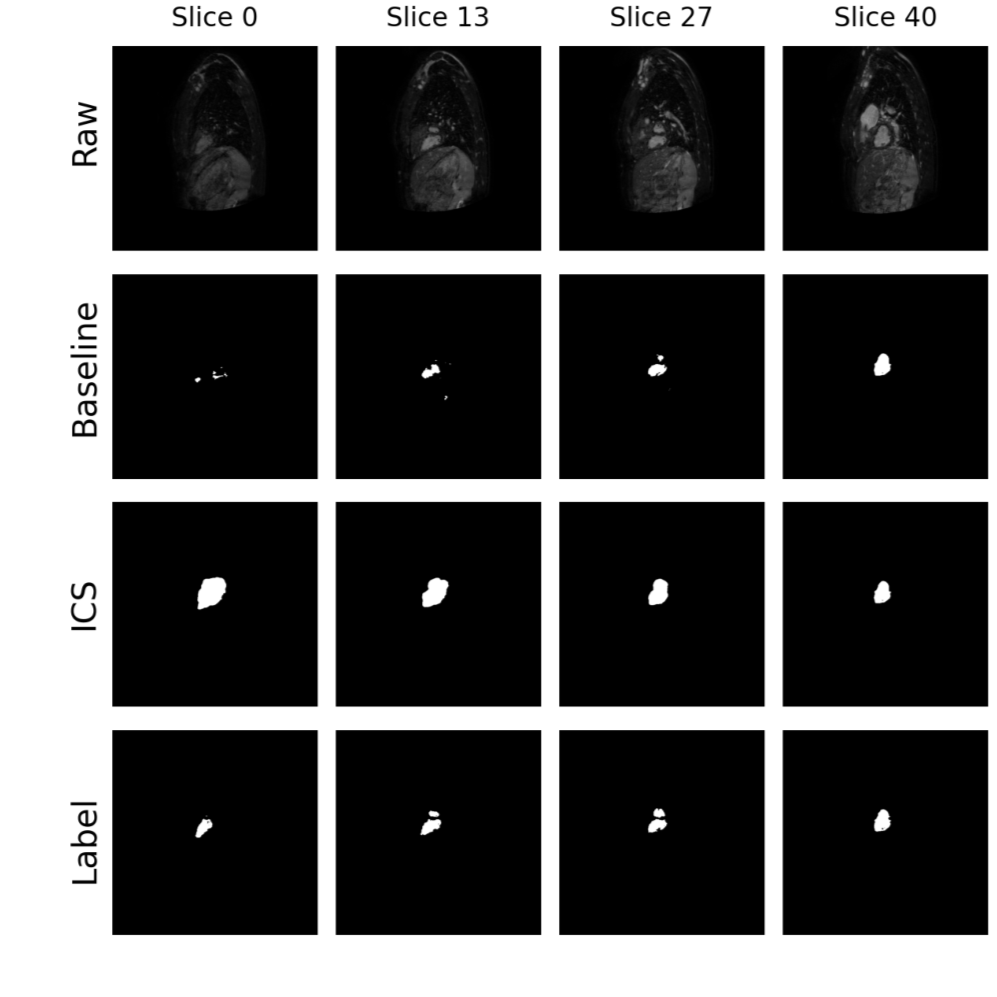
\includegraphics[width=\linewidth]{LV.png}

        \column{0.45\textwidth}
            \centering
            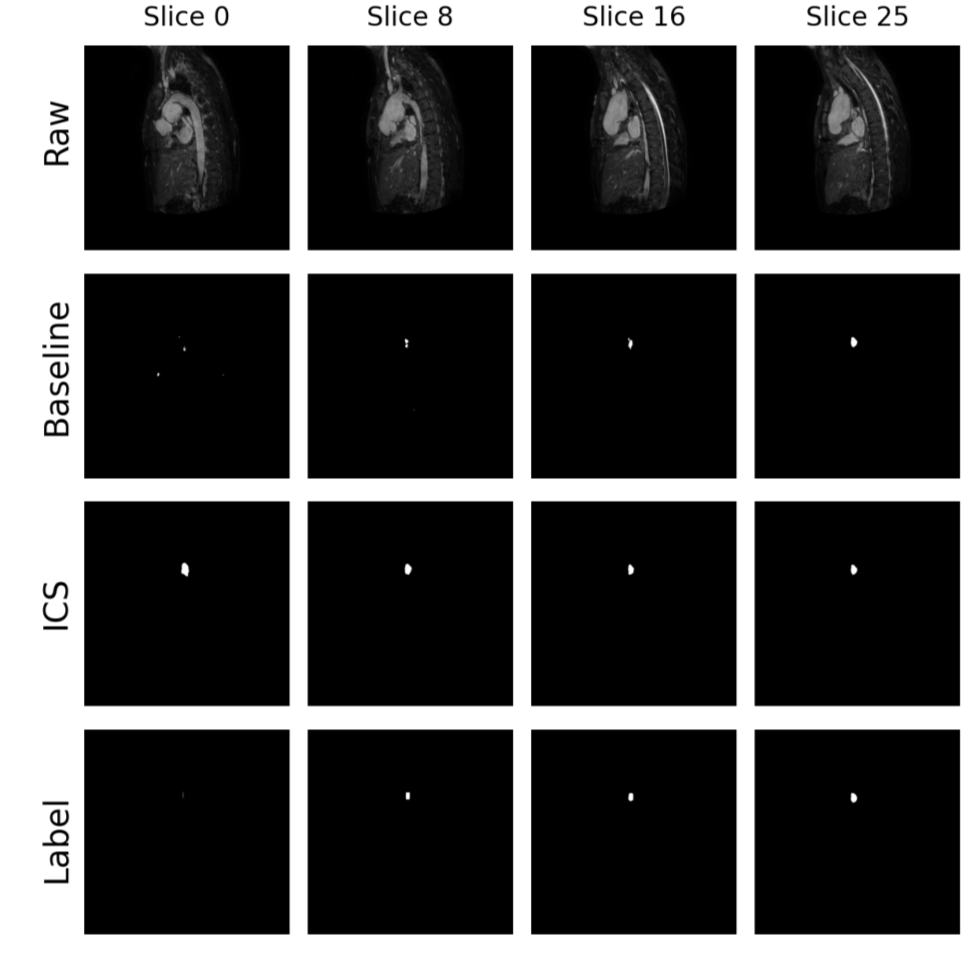
\includegraphics[width=\linewidth]{PA.png}
    \end{columns}

\end{frame}

\subsection{The DSC score against each slice}
\begin{frame}[label=paLVslide]
    \frametitle{Pulmonary Artery and Left Ventricle}
    \framesubtitle{DSC Score Slice wise}
    \centering
    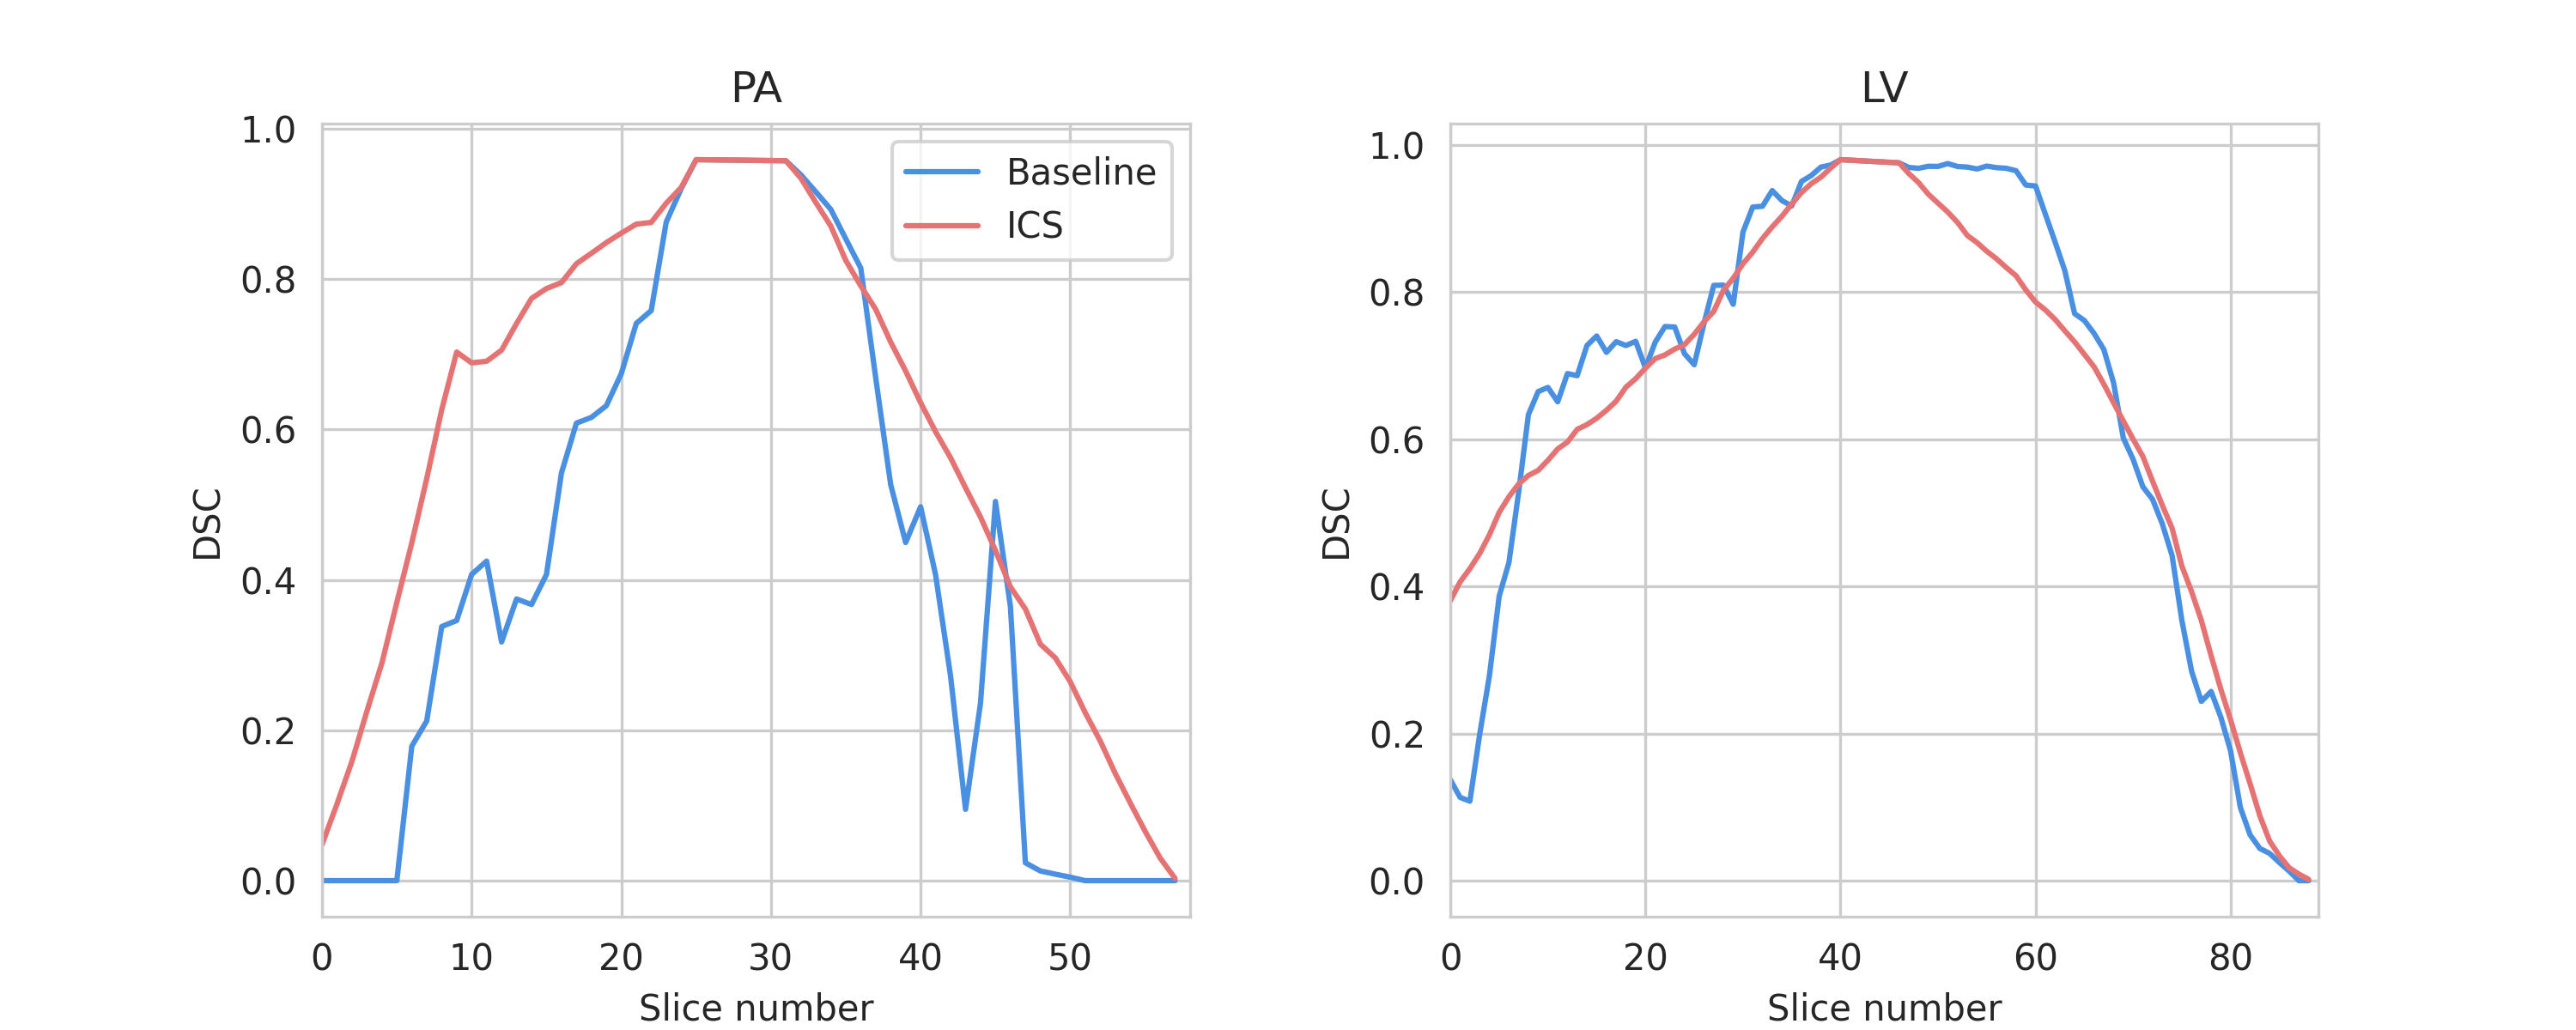
\includegraphics[width=1.1\textwidth]{fig6.png}
\end{frame}

\subsection{Effect of Initial Slice Position}
\begin{frame} 
    \frametitle{Effect of Initial Slice Position}
    \framesubtitle{Line Plot of Aorta and Pulmonary Artery}
    \centering
    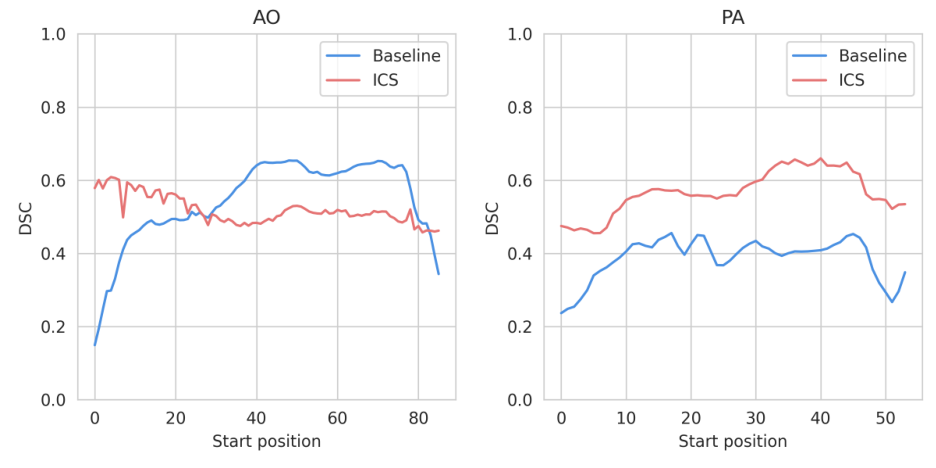
\includegraphics[width=0.88\textwidth]{fig8.png}
\end{frame}

\section{Discussion \& Conclusion}
\begin{breakframe}
    Discussion \& Conclusion
\end{breakframe}

\subsection{Discussion \& Limitations}
\begin{frame}[label=disc1]
    \frametitle{Discussion}
    \framesubtitle{Strengths and Limitations}

    \begin{columns}[T]
        \column{0.48\textwidth}
            \vspace{0.3cm}
            \begin{itemize}
                \item ICS remains consistently accurate on complex structures.

                \vspace{0.5em}
                \item Often prone to over-segmenting certain anatomical regions.

                \vspace{0.5em}
                \item Initial support slice distance heavily degrades accuracy.
            \end{itemize}

        \column{0.48\textwidth}
            \vspace{0.2cm}
            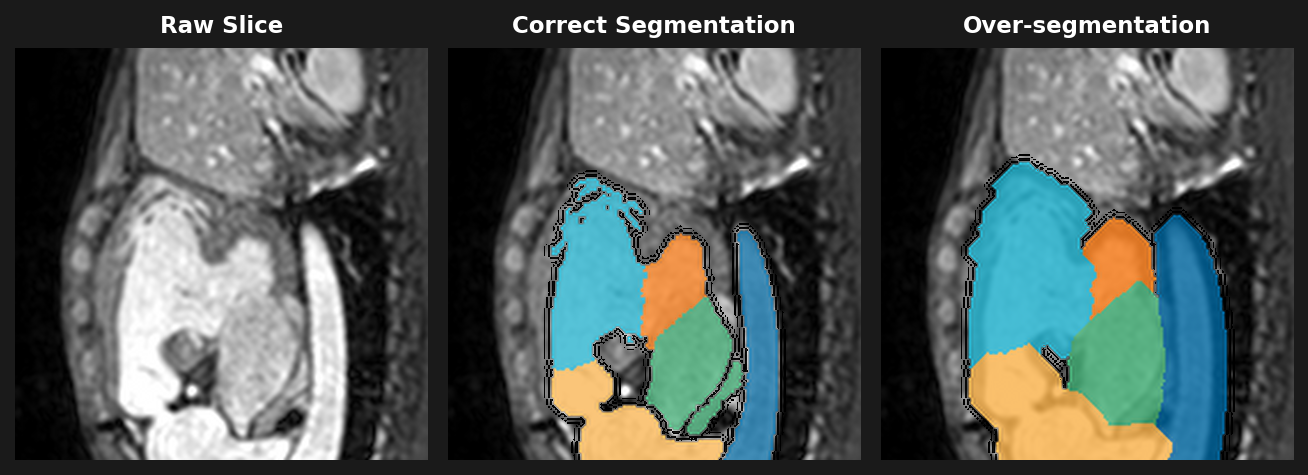
\includegraphics[width=\linewidth]{images/disc_comparison.png}

    \end{columns}

    \vspace{0.3em}
    {\tiny\textcolor{grau2}{Source: \href{https://arxiv.org/abs/2412.13299}{Takaya \& Yamamoto, In-Context Learning for Medical Image Segmentation, 2025}}}

\end{frame}

% Questions Slide
\begin{frame}
    \frametitle{}
    \framesubtitle{}

    \vspace*{\fill}
    \centering

    {\LARGE\bfseries\textcolor{orange1}{Thank you for your attention!}}

    \vspace{0.6em}

    {\large\textcolor{grau1}{I am open to your questions!}}

    \vspace{0.5em}

    
\includegraphics[height=5.2em]{text.png}

    \vspace*{\fill}

\end{frame}

% Thank You
\begin{thankyouframe}
\end{thankyouframe}

\begin{frame}
    \frametitle{Effect of Support Slice Count}
    \framesubtitle{DSC vs. Number of Initial Support Slices}
    \centering
    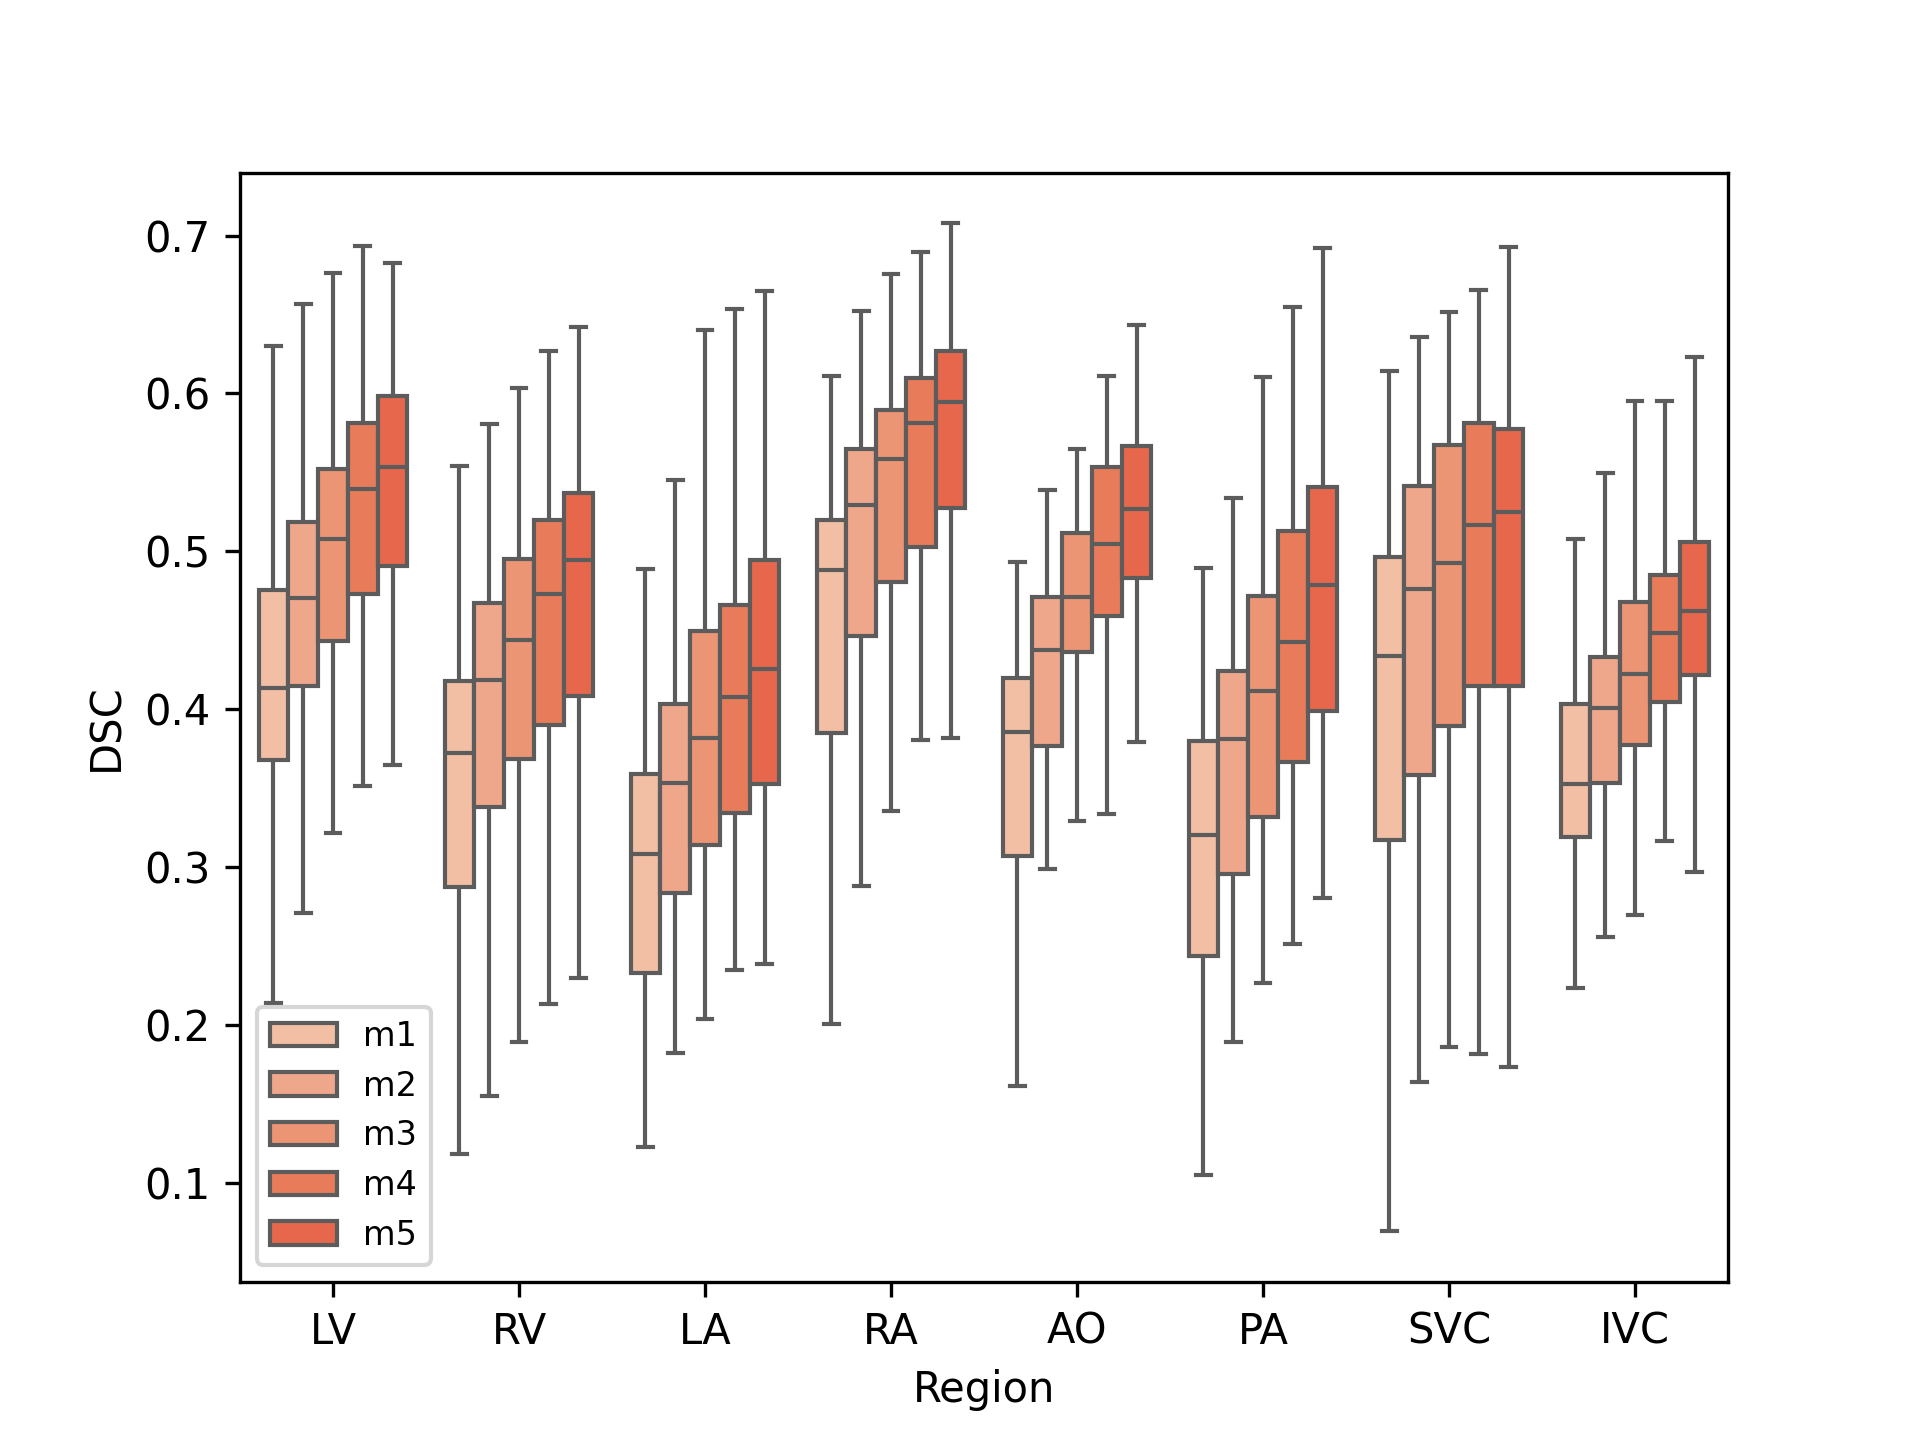
\includegraphics[width=\textwidth, height=0.82\textheight, keepaspectratio]{fig7.png}
\end{frame}

\subsection{ICS Algorithm}
\begin{frame}
    \frametitle{ICS Algorithm }
    \framesubtitle{Initialization \& Forward Pass}

    {\small
    \textbf{Require:} Volume $V$, InitialSupportSet, UniverSeg, max size $m$, Augment()

    \vspace{0.5em}
    \textbf{Initialize:} ForwardSupportSet $\leftarrow$ InitialSupportSet\\
    \phantom{\textbf{Initialize:}} BackwardSupportSet $\leftarrow$ InitialSupportSet

    \vspace{0.6em}
    \textcolor{cyan1}{\textbf{Forward pass}} ($i = \max(c_k)$ to $n$):
    \begin{enumerate}\itemsep6pt
        \item Query $\leftarrow$ slice$_i$
        \item $\hat{y} \leftarrow$ UniverSeg(Query, Augment(ForwardSupportSet))
        \item Append $(\text{slice}_i, \hat{y})$ to ForwardSupportSet
        \item If $|$ForwardSupportSet$| > m$: remove oldest entry
    \end{enumerate}
    }

\end{frame}

\begin{frame}
    \frametitle{ICS Algorithm }
    \framesubtitle{Backward Pass \& Key Properties}

    {\small
    \textcolor{lila1}{\textbf{Backward pass}} ($i = \min(c_k)$ down to $1$):
    \begin{enumerate}\itemsep6pt
        \item Query $\leftarrow$ slice$_i$
        \item $\hat{y} \leftarrow$ UniverSeg(Query, Augment(BackwardSupportSet))
        \item Append $(\text{slice}_i, \hat{y})$ to BackwardSupportSet
        \item If $|$BackwardSupportSet$| > m$: remove oldest entry
    \end{enumerate}

    \vspace{0.5em}
    \textbf{Return:} ForwardPredictedLabels, BackwardPredictedLabels

    \vspace{0.6em}
    \textcolor{orange1}{\textbf{Rolling window}} ($m = 5$): oldest entries discarded to keep context spatially local.
    Augmentation: rotations 90°/180°/270° at each step.
    UniverSeg weights remain \textbf{frozen} throughout.
    }

\end{frame}


\subsection{References}
\begin{frame}[label=refslide]
    \frametitle{References}
    \framesubtitle{Related Works}

    {\tiny
    \begin{enumerate}
        \item Takaya E., Yamamoto S. \textit{In-Context Learning for Medical Image Segmentation.}
              arXiv:2412.13299, 2025.
              \url{https://arxiv.org/abs/2412.13299}

        \item Pham D.L. et al. \textit{Current Methods in Medical Image Segmentation.}
              Annual Review of Biomedical Engineering, 2000.
              \url{https://pubmed.ncbi.nlm.nih.gov/11701515/}

        \item Azad R. et al. \textit{Medical Image Segmentation Review: The Success of U-Net.}
              IEEE TPAMI, 2024.
              \url{https://ieeexplore.ieee.org/document/10643318}

        \item Dong Q. et al. \textit{A Survey on In-context Learning.}
              arXiv:2301.00234, 2023.
              \url{https://arxiv.org/abs/2301.00234}

        \item von Oswald J. et al. \textit{Transformers Learn In-Context by Gradient Descent.}
              ICML, 2023.
              \url{https://arxiv.org/abs/2212.07677}

        \item Jiao R. et al. \textit{Learning with Limited Annotations: A Survey on Deep
              Semi-Supervised Learning for Medical Image Segmentation.}
              arXiv:2207.14191, 2022.
              \url{https://arxiv.org/abs/2207.14191}

        \item Butoi V. et al. \textit{UniverSeg: Universal Medical Image Segmentation.}
              ICCV, 2023.
              \url{https://universeg.csail.mit.edu/}
    \end{enumerate}
    }

    \vspace{0.5em}
    \begin{alertblock}{}
        \small\textbf{Presenter's Declaration:} All scientific work, ideas, experiments and results presented in this talk belong entirely to \textbf{Takaya E.\ and Yamamoto S.} This presentation is solely an academic explanation of their published research. No part of this work is claimed or owned by the presenter.
    \end{alertblock}

    \vspace{0.3em}
    {\tiny\textcolor{grau2}{AI Declaration: Generative AI tools (ChatGPT) were used for idea generation and grammar correction.}}

\end{frame}

\end{document}
